% !TEX program = lualatex
\documentclass[a4paper,11pt]{ltjsarticle}

\usepackage{amsmath,amssymb}
\usepackage{booktabs}
\usepackage{graphicx}
\usepackage{longtable}
\usepackage{array}
\usepackage{multirow}
\usepackage{float}
\usepackage[margin=22mm]{geometry}
\usepackage[hidelinks]{hyperref}

\newcommand{\He}{\ensuremath{{}^{3}\mathrm{He}}}
\newcommand{\teq}{t_{\mathrm{eq}}}
\newcommand{\RNET}{R_{\mathrm{NET}}}
\newcommand{\eSpk}{\varepsilon S_{\mathrm{peak}}}
\newcommand{\flux}{\mathrm{cm^{-2}\,s^{-1}}}
\newcommand{\gcm}{\mathrm{g\,cm^{-2}}}
\newcommand{\sci}[2]{\ensuremath{#1\times10^{#2}}}

\title{地下での中性子フラックスの測定\\[4pt]
\large ——等価コンクリート厚に対する熱・MeV 中性子の深度依存と\\ミューオン起源中性子による解釈——}
\author{KEK サマーチャレンジ 2026\quad 9班\\[6pt]
\small 学生：川嶋 宥翔（名古屋大学）・鈴江 春樹（明治大学）・高橋 源太（金沢大学）\\
\small 戸田 日々輝（東京大学）・西之原 純輝（宮崎大学）\\[2pt]
\small 教員：岩瀬 広・岸本 祐二・大山 隆宏・飯島 和彦\\[2pt]
\small TA：星野 稔・落合 勇稀・小川 拓泰・小林 海景}
\date{2026年9月25日}

\begin{document}
\maketitle

\begin{abstract}
昨年度の9班は，大気中の中性子フラックスが標高に対して指数関数的に変化することを示した。
本研究ではその続きとして，地表より下で中性子フラックスがどう変化するかを調べた。
KEK つくばキャンパスの地上と，等価コンクリート厚 $\teq=57$--$525$\,cm の地下施設7か所で，
\He 比例計数管4台（裸管で熱中性子，ポリエチレン減速材付きで MeV 中性子）により中性子捕獲ピークの計数率を測り，絶対フラックスを求めた。

地上の熱中性子フラックス $(1.69\pm0.04)\times10^{-3}\,\flux$ は，較正方法の違いによる数十\% の不確かさの範囲で昨年度の値と整合した。
一方，地下では $\teq=300$\,cm でも地上の約 20\%，525\,cm でも約 10\% が残り，
単純指数減衰（$\lambda=60$\,cm）の予測を KEKB で約 700 倍上回った。
この成分の起源として地下まで届く宇宙線ミューオンが作る中性子を考え，
PHITS で宇宙線の成分ごとに中性子の深さ分布を計算したところ，$\teq\ge300$\,cm の中性子の 72--97\% がミューオン起源で，その大部分が負ミューオンの原子核捕獲によるものであった。
さらに PHITS で検出器の応答関数を求め，地点ごとの遮蔽と部屋を含む体系で計数率を較正なしに予測したところ，PF・BT・PS の大径裸管（D1）は実測と 15\% 以内で一致した（ただし D1 のピーク窓の割合を小径管の値で代用した仮定の下での結果である）。
ただし深い地点の一部では実測が予測の約2倍以上あり，ミューオン起源の成分を約3倍にすると合う。
この差の原因は，地点の3次元の構造と減速材付き管の応答の両面から確かめる必要がある。
\end{abstract}

\newpage
\begingroup
\linespread{0.92}\small\selectfont
\tableofcontents
\endgroup
\newpage

%======================================================================
\section{序論}
%======================================================================

\subsection{宇宙線由来の中性子}

一次宇宙線（主に陽子）が大気上層の原子核と衝突すると，大気シャワーが起こり，
二次粒子として陽子・中間子・ミューオン・電子・光子・中性子が地表に降り注ぐ。
電荷をもたない中性子は，空気や地面の原子核との衝突でエネルギーを失い，
最終的に熱エネルギー程度（$\sim0.025$\,eV）まで減速される。
本研究では中性子を運動エネルギーで次のように呼び分ける。

\begin{itemize}
  \item \textbf{熱中性子}：$\sim0.025$\,eV の熱平衡領域。\He の捕獲断面積が大きく，裸の \He 管で効率よく検出できる。
  \item \textbf{MeV 中性子}：$\sim1$\,MeV 前後。ポリエチレン（PE）減速材で熱化させてから \He 管で検出する。
  \item GeV 中性子：大気シャワーの高エネルギー成分。\He 検出器では直接測れない。
\end{itemize}

\subsection{昨年度（2025年度 9班）の結果}

昨年度の9班は，今年度の d1 と同型の \He 管（寸法から同一個体の可能性が高い）を用いて，
KEK（管理棟・屋外，標高約 30\,m），筑波山（観測点約 800\,m），日光白根山（観測点約 2000\,m）で
熱中性子と MeV 中性子のフラックスを測定した\cite{lastyear}。
図\ref{fig:lastyear}に示すように，フラックスは標高とともに指数関数的に増加し，
\begin{equation}
  \lambda_{\mathrm{air}} = \frac{\Delta h}{\ln(\phi_2/\phi_1)}
\end{equation}
で定義した空気中の減衰長（昨年度の報告では平均自由行程と呼んだ）は，管理棟1階（$\phi_1=1.83\times10^{-3}\,\flux$）と
白根山（$\phi_2=7.10\times10^{-3}\,\flux$，$\Delta h=2000$\,m と近似）の組から
熱中性子で $\lambda_{\mathrm{air}}=1475\pm29$\,m（空気の密度を一様に $1.0\times10^{-3}$\,g\,cm$^{-3}$ として質量厚さに換算すると $\Lambda=147.5\,\gcm$），
MeV 中性子で約 1000\,m（$\Lambda\approx100\,\gcm$）であった（表\ref{tab:lastyear}）。
昨年度の裸管の実効面積は，黒鉛パイルでの実測から $\varepsilon S\approx88$--92\,cm$^2$（177--941\,keV の広い窓）とされている\cite{lastyear}。

\begin{figure}[htbp]
  \centering
  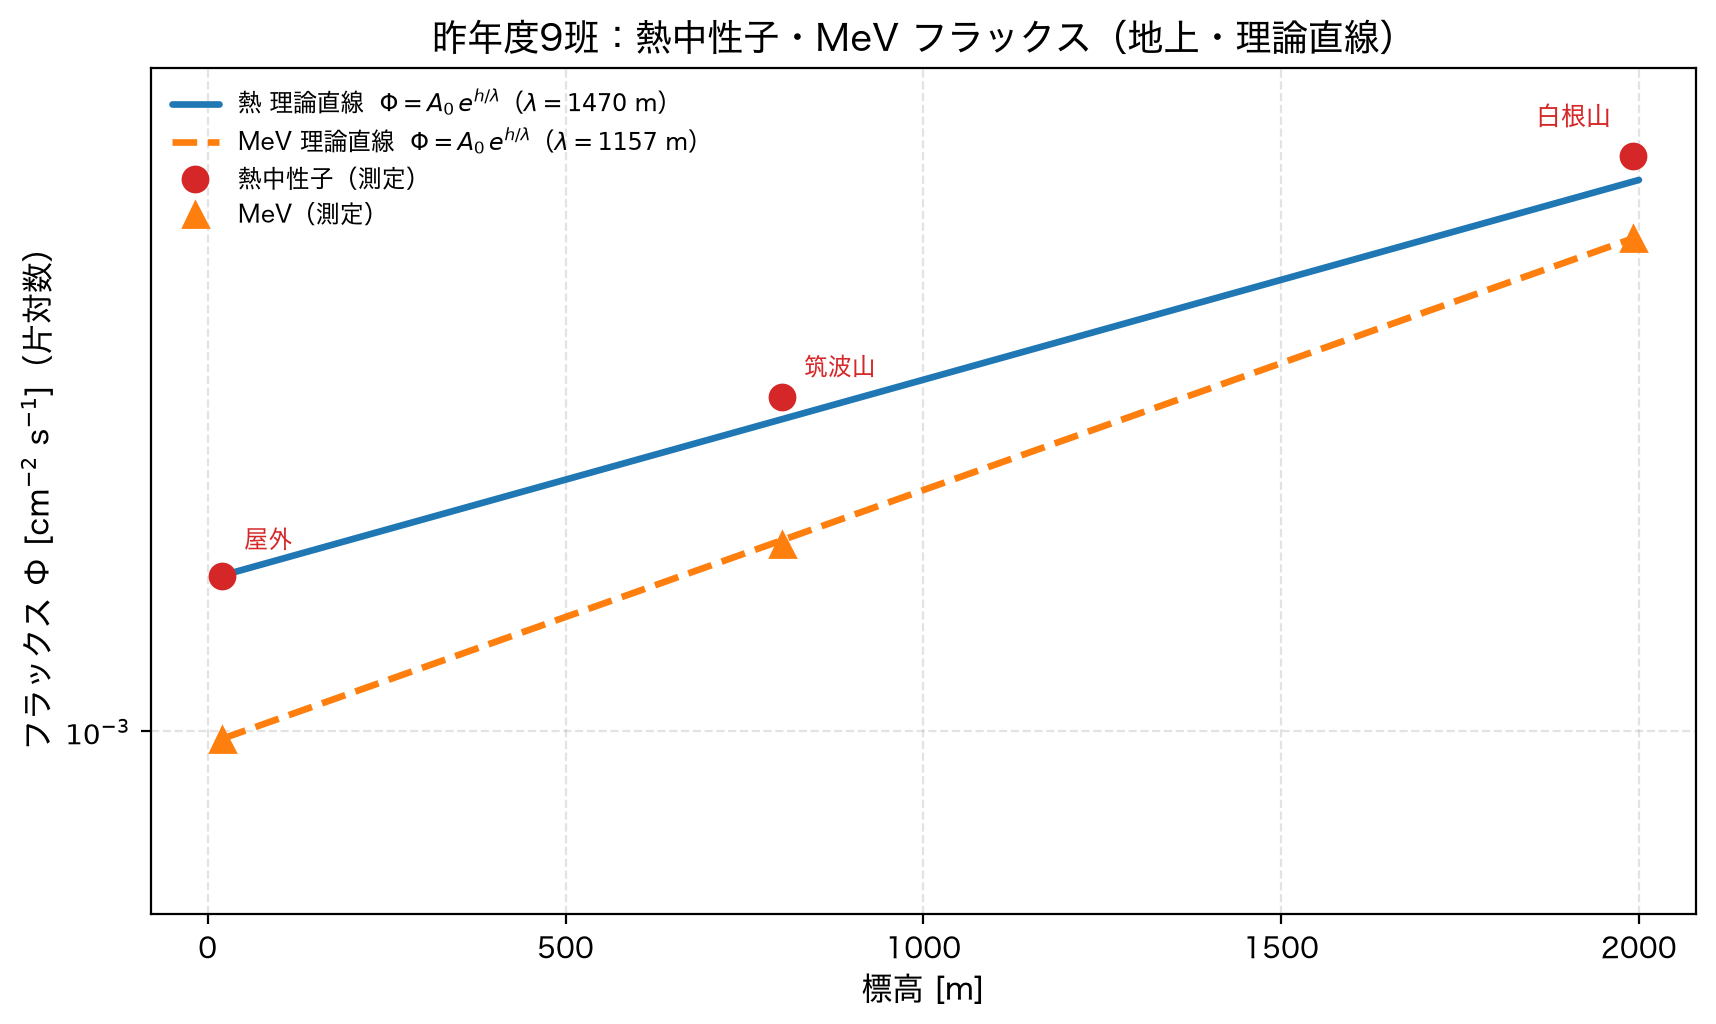
\includegraphics[width=0.78\linewidth]{figures/fig01_lastyear_altitude.png}
  \caption{昨年度9班の標高依存の結果\cite{lastyear}。縦軸は片対数。実線・破線は $\phi=A_0e^{h/\lambda}$。}
  \label{fig:lastyear}
\end{figure}

\begin{table}[htbp]
  \centering
  \caption{昨年度の熱中性子（裸管）の測定値と減衰長\cite{lastyear}}
  \label{tab:lastyear}
  \begin{tabular}{lrrrr}
    \toprule
    地点 & 計数 $N$ & 時間 $t$ [s] & 計数率 $R$ [s$^{-1}$] & $\phi$ [$\flux$] \\
    \midrule
    管理棟2階 & 7162 & 35793 & 0.200 & $2.25\times10^{-3}$ \\
    管理棟1階 & 7035 & 43106 & 0.163 & $1.83\times10^{-3}$ \\
    プレハブ   & 3012 & 11672 & 0.258 & $2.90\times10^{-3}$ \\
    屋外      & 1688 & 10807 & 0.156 & $1.70\times10^{-3}$ \\
    筑波山    &  803 &  2889 & 0.278 & $3.12\times10^{-3}$ \\
    白根山    & 1745 &  2759 & 0.632 & $7.10\times10^{-3}$ \\
    \midrule
    \multicolumn{5}{l}{管理棟1階 $\to$ 白根山：熱 $\lambda_{\mathrm{air}}=1475$\,m（$\Lambda=147.5\,\gcm$），MeV $\lambda_{\mathrm{air}}\approx1000$\,m} \\
    \bottomrule
  \end{tabular}\\[2pt]
  \footnotesize 屋外の行は昨年度の発表スライドの値（公開用の表では空欄）。昨年度の最終発表では，地表の代表値として別の集計の $1.33\times10^{-3}\,\flux$ も示されている。
\end{table}

\subsection{本研究の目的}

昨年度の結果を受け，本研究では次の問いを立てた。

\begin{quote}
  \textbf{地表より下（コンクリートや土の遮蔽下）でも，中性子フラックスは深さに対して同じように指数減衰するのか。}
\end{quote}

KEK には，加速器を収めるために深さ（遮蔽厚）の異なる地下トンネル・地下室が構内に多数ある。
これらを巡って測定すれば，1回のキャンペーンで遮蔽厚 0--5\,m 超の深度依存を追うことができる。
測定期間中（夏季停止期間）は全加速器のビームが停止しており，加速器起源の中性子は存在しない前提で解析した。

%======================================================================
\section{原理}
%======================================================================

\subsection{\He 比例計数管による中性子検出}

\He 比例計数管は，管内の \He ガスが中性子を捕獲する反応
\begin{equation}
  {}^{3}\mathrm{He} + n \;\to\; p + {}^{3}\mathrm{H} + 764\ \mathrm{keV}
\end{equation}
を利用する。放出エネルギー $Q=764$\,keV は，運動量保存により陽子（573\,keV）とトリトン（191\,keV）に反対向きに分配され，
両者がガスを電離して生じた電荷を比例増幅して読み出す。
熱中性子に対する捕獲断面積は約 5330\,b と大きく，断面積は概ね $1/v$ に比例するため，
低エネルギーの中性子ほど検出されやすい\cite{Knoll}。

両粒子がガス中で全エネルギーを落とせば 764\,keV の\textbf{全吸収ピーク}が現れる。
反応点が管壁に近いと一方の粒子が壁に入ってエネルギーの一部しか落とさないため，
191\,keV（トリトンのみ）から 764\,keV までの連続成分（\textbf{壁効果}）が生じる。
典型的なスペクトルを図\ref{fig:spec}に示す。
本解析では主に 764\,keV の全吸収ピーク（peak ROI）の正味計数率を用いた。

\subsection{フラックスの定義}

単位時間・単位面積あたりに通過する中性子数をフラックス $\phi$ [$\flux$] とすると，
検出器の計数率 $R$，検出効率 $\varepsilon$，有効面積 $S$ の間には $R=\varepsilon S\phi$ が成り立つ。したがって
\begin{equation}
  \phi = \frac{R}{\varepsilon S}
  \label{eq:flux}
\end{equation}
である（昨年度と同じ定義）。本解析では $R$ を peak ROI の正味計数率 $\RNET$，$\varepsilon S$ を peak ROI に対する実効面積 $\eSpk$ とした。
裸管の $\phi$ は \He の $1/v$ 応答で重み付けした「熱中性子等価フラックス」であり，熱外中性子の寄与も一部含む。
PE 付き管の $\phi$ は，減速材で熱化された MeV 領域中性子に感度をもつ量として扱う。

\subsection{等価コンクリート厚}

中性子が遮蔽物中で減るのは原子核との反応によるので，反応の起こりやすさは通り道にある原子核の数，
すなわち\textbf{質量厚さ} $X=\rho t$ [$\gcm$] で決まる。
原子核の反応断面積の経験式 $\sigma\approx45A^{0.7}$\,mb から，反応を1回起こすまでの平均自由行程（相互作用長）は
\begin{equation}
  \Lambda_i = \frac{A}{N_A\sigma} \approx 37\,A^{0.3}\ \ \gcm
\end{equation}
となり，質量数 $A$ が 200 倍変わっても $\Lambda$ は約 5 倍（$200^{0.3}\approx4.9$）しか変わらない\cite{kyozai}。
組成の混合則 $1/\Lambda=\sum_i w_i/\Lambda_i$（$w_i$ は質量分率）を適用すると，
コンクリート（O 53\%，Si 34\%，Ca 4\%，Al 3\%，H 1\%）で $\Lambda\approx92\,\gcm$（教材の値は $90.2\,\gcm$），
土（O 50\%，Si 27\%，Al 7\%，Fe 4\%，H 2\%）で $\Lambda\approx93\,\gcm$ となり，差は約 1\% である。
したがって土とコンクリートは質量厚さで1本の軸にまとめてよく，本研究では横軸を
\begin{equation}
  \teq = \frac{X}{\rho_c} = \frac{1}{\rho_c}\sum_{k}\rho_k t_k,
  \qquad \rho_c = 2.3\ \mathrm{g\,cm^{-3}}
  \label{eq:teq}
\end{equation}
の\textbf{等価コンクリート厚}に統一した。土の密度は KEK の地層区分に従い，
関東ローム 1.35，常総層 1.65，下総層 1.85\,g\,cm$^{-3}$ とした。
なお，地下の中性子フラックスの文献\cite{FabrykaMartin1988}で用いられる水当量深さとは，$1\ \mathrm{m.w.e.}=100\,\gcm\approx43$\,cm（コンクリート）で換算できる。

\subsection{単純指数減衰による予測}

昨年度の大気中の結果を踏まえ，地下でもまず
\begin{equation}
  \phi(\teq) = A_0\,\exp\!\left(-\frac{\teq}{\lambda_c}\right)
  \label{eq:simple}
\end{equation}
の単純指数減衰を予測とした。$A_0$ は地上の実測値である。
減衰長 $\lambda_c$ として，教材の混合則による $\Lambda_c=90.2\,\gcm$（$\lambda_c=39.2$\,cm）と，
$\lambda_c=60$\,cm（$\Lambda\approx138\,\gcm$。昨年度の大気中の値 $100$--$147.5\,\gcm$ の範囲にある）の2通りを考えた。
ただし前者は反応1回までの平均距離であり，実際には反応で生じた二次中性子がさらに反応を起こすため，フラックスの減衰長は相互作用長より長くなる。
例えば岩石中の宇宙線核種の生成率には $\Lambda\approx160\,\gcm$ が標準的に用いられる\cite{Gosse2001}。
教材\cite{kyozai}は，地下で測る MeV 中性子は検出器の近く（$\sim11$\,cm 以内）で高エネルギー中性子から生成されたものであり，
その深度依存は親である高エネルギー中性子の減衰長で決まる，という単一指数の描像を与えている。

%======================================================================
\section{実験}
%======================================================================

\subsection{装置}

測定系は \He 比例計数管，プリアンプ，整形アンプ，MCA（Amptek MCA8000D，512\,ch），PC からなる。
MCA は波高分布をチャンネルごとに積算し，ライブタイム（不感時間を除いた実測定時間）とともに記録する。
使用した検出器を表\ref{tab:detectors}に示す。大文字 D は大径管，小文字 d は小径管，末尾 1 は裸管，2 は PE 減速材付きを表す。

\begin{table}[htbp]
  \centering
  \caption{使用した \He 比例計数管}
  \label{tab:detectors}
  \small
  \begin{tabular}{llllp{0.24\linewidth}l}
    \toprule
    記号 & 対象 & 型番（シリアル） & 有効長 & 減速材 & メーカー感度 \\
    \midrule
    D1 & 熱 & RS-P4-3224-201（SN1715） & 60.96\,cm & なし & 450\,cps/nv \\
    D2 & MeV & 大径管 & 同上 & PE 容器（外径 29／内径 15／高さ 80\,cm） & --- \\
    d1 & 熱 & P4-1613-203（SN2162） & 43.18\,cm & なし & 123\,cps/nv \\
    d2 & MeV & 小径管 & 同上 & PE 筒（厚さ 5\,cm） & --- \\
    \bottomrule
  \end{tabular}\\[2pt]
  \footnotesize cps/nv は熱中性子フラックス 1\,$\flux$ あたりの計数率で，$\varepsilon S$ [cm$^2$] に等しい。
\end{table}

\subsection{測定地点と遮蔽}

測定地点と遮蔽層の構成を表\ref{tab:sites}に示す。
遮蔽層の厚さは各施設の図面と KEK の地層柱状図から読み取った垂直方向の値で，
式\eqref{eq:teq}で等価コンクリート厚に換算した。

\begin{table}[htbp]
  \centering
  \caption{測定地点と遮蔽層（垂直積層）}
  \label{tab:sites}
  \footnotesize
  \begin{tabular}{lrrrrrl}
    \toprule
    地点 & コンクリート & 土 & $X$ & $\teq$ & 水当量 & 備考 \\
         & [cm] & [cm] & [$\gcm$] & [cm] & [m.w.e.] & \\
    \midrule
    地上（屋外） & 0 & 0 & 0 & 0 & 0 & 管理棟南側，基準点 \\
    管理棟2階・1階 & --- & --- & --- & （0） & --- & 屋内（参考） \\
    Linac テストホール & 57 & 0 & 131 & 57 & 1.3 & \\
    PF & 105 & 0 & 242 & 105 & 2.4 & リングトンネル内，天井スラブ直下 \\
    放射線棟 BT & 60 & 220 & 435 & 189 & 4.4 & 土はローム層 \\
    Linac3 & 300 & 0 & 690 & 300 & 6.9 & ATF 加速管区間 \\
    K2K ビームライン & 444 & 0 & 1021 & 444 & 10.2 & 等価値 \\
    PS & 480 & 0 & 1104 & 480 & 11.0 & 等価値 \\
    KEKB & 80 & 670 & 1209 & 525 & 12.1 & ローム 350＋常総 200＋下総 120\,cm \\
    \bottomrule
  \end{tabular}
\end{table}

\subsection{測定の経過}

測定は 2026年8月18日から26日まで行った。
8/18--19 に管理棟（2階終夜 14.5\,h，1階 4.9\,h）と地上を測定して地表の基準を取り，
8/19--8/26 に地下施設を順に巡った（各地点 2.7--21.8\,h）。
8/22 には熱中性子管理棟の黒鉛パイル（Am-Be 線源）で検出器の較正測定を行った。
解析に用いた測定の一覧を\ref{app:runs}に示す。
同一地点では原則として大径・小径の2台を並べて同時に測定し，検出器間の整合性を確認できるようにした。

%======================================================================
\section{解析}
%======================================================================

\subsection{スペクトルと peak ROI}

図\ref{fig:spec}に D1 の地上と Linac3 のスペクトルを示す。
ch 0 は ADC のオーバーフロー（全計数の約半分）で情報をもたないため除外した。
低チャンネル側には閾値付近のノイズ・$\gamma$ 線の成分が大きく立ち上がり，
191\,keV から 764\,keV にかけて壁効果の連続成分，764\,keV に全吸収ピークが見える。
ピーク位置はアンプ設定により SN1715 で ch 340 付近または ch 385 付近，SN2162 で ch 389 付近にあり，
peak ROI はスペクトルごとにピークを中心とする約 52\,ch 幅の窓として自動決定した。

\begin{figure}[htbp]
  \centering
  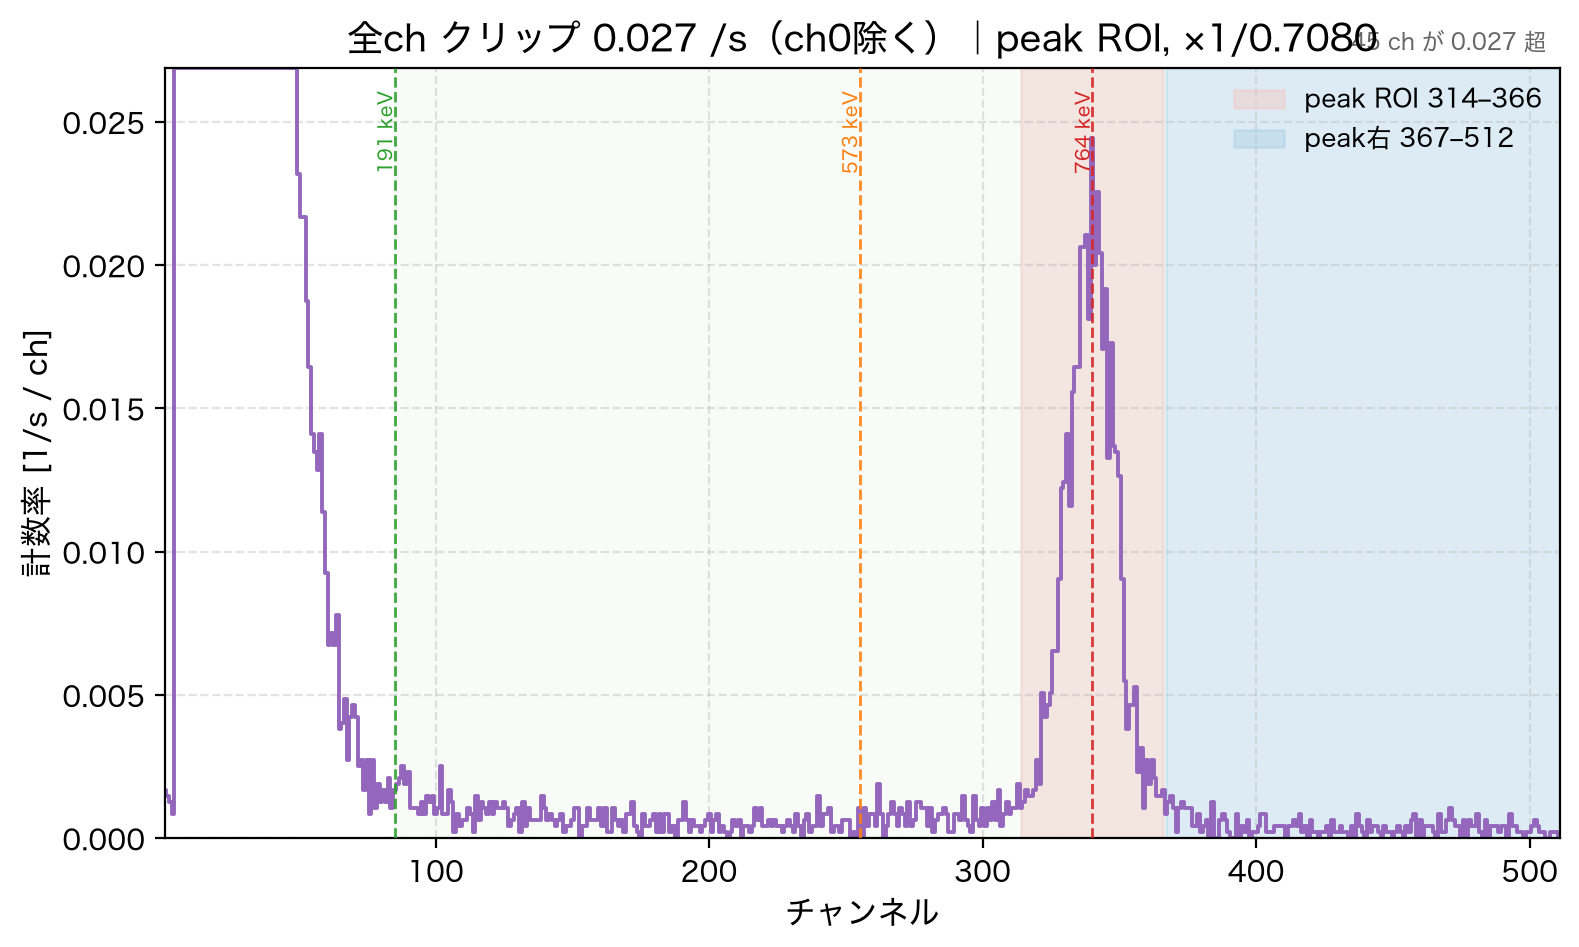
\includegraphics[width=0.49\linewidth]{figures/fig02_spectrum_D1_ground.png}\hfill
  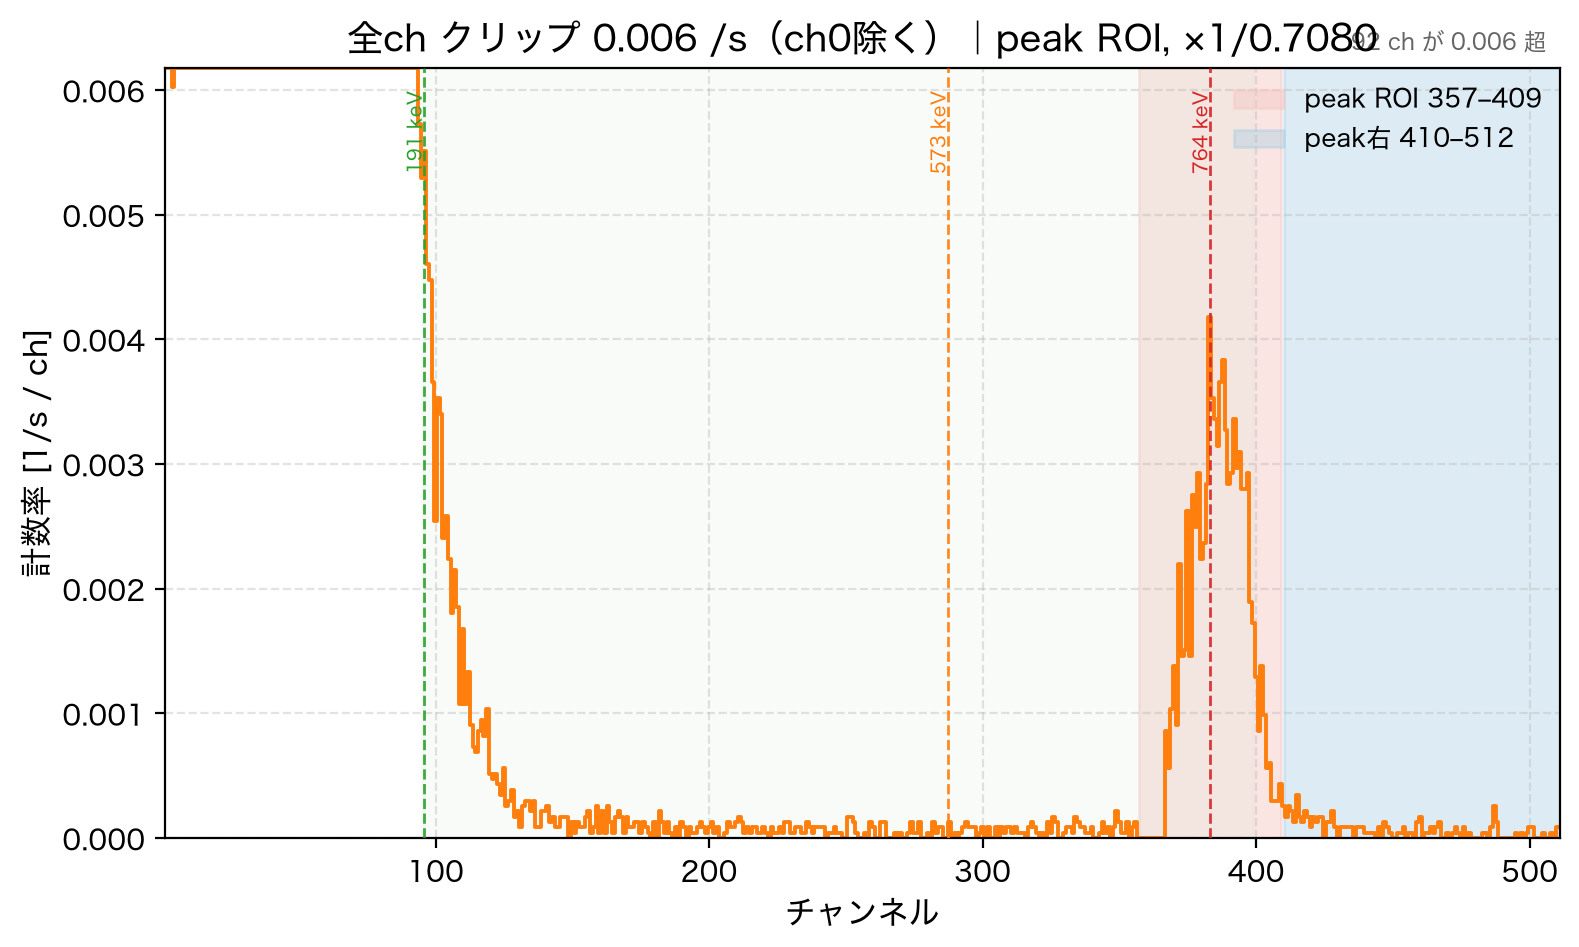
\includegraphics[width=0.49\linewidth]{figures/fig03_spectrum_D1_linac3.png}
  \caption{D1 のスペクトル（ch 0 除外，縦軸は計数率）。左：地上（ライブタイム 4748\,s），右：Linac3（23223\,s，部分補正後）。
  縦線は 191\,keV（壁効果の下端），573\,keV，764\,keV（全吸収ピーク）。赤の帯が peak ROI，青の帯がピーク右側の側帯。}
  \label{fig:spec}
\end{figure}

\subsection{正味計数率}

peak ROI 内の総計数 $N_{\mathrm{GROSS}}$ から，ピーク左右の側帯（sideband）で見積もった背景 $N_{\mathrm{BG}}$ を差し引き，
\begin{equation}
  N_{\mathrm{NET}} = N_{\mathrm{GROSS}} - N_{\mathrm{BG}},\qquad
  \RNET = \frac{N_{\mathrm{NET}}}{t_{\mathrm{live}}},\qquad
  \delta\RNET = \frac{\sqrt{N_{\mathrm{GROSS}}+N_{\mathrm{BG}}}}{t_{\mathrm{live}}}
\end{equation}
とした。$t_{\mathrm{live}}$ はライブタイムである。右側帯が使えない場合は左側帯のみの水平背景を用いた。

\subsection{スペクトルの部分補正}
\label{sec:partial}

地下の一部の測定では低チャンネルのノイズがピーク左裾まで漏れ込み，側帯背景が正しく引けなかった。
そこで，ノイズの少ない黒鉛パイルでの熱中性子スペクトルから，peak ROI の正味計数のうちカットチャンネル以上に含まれる割合 $f$ を求め，
問題のあるスペクトルではカット未満のチャンネルを捨て，カット以上を $1/f$ 倍した（以下，部分補正と呼ぶ）。
\begin{equation}
  N_{\mathrm{NET}}^{\mathrm{corr}} = \frac{N_{\mathrm{NET}}(\mathrm{ch}\ge \mathrm{cut})}{f},
  \qquad f_{\mathrm{large}}=0.708\ (\mathrm{D1/D2}),\quad f_{\mathrm{small}}=0.668\ (\mathrm{d1/d2})
\end{equation}
ピークがきれいなスペクトル（カット以上の割合が 0.84 以上で左漏れが弱いもの）には補正を適用しない。
補正を適用したのは Linac3・PS・KEKB・テストホールの D1，Linac3 の D2，Linac3・PS・テストホールの d1，地上・Linac3・KEKB の d2 である。
なお，本報告の作成途中で，解析の途中段階のデータ統合処理において，補正済みのスペクトルにもう一度この補正がかかっていた（実質 $1/f^2$ 倍）ことが判明した。
このため上記の 11 点の $\RNET$ は 1.41--1.50 倍過大になっていた。本報告の数値と図は，補正前のスペクトルから補正を1回だけかけ直した値にすべて改めてある。

\subsection{検出効率（実効面積）の較正}
\label{sec:calib}

\paragraph{裸管（D1，d1）}
中性子は電荷をもたず，核反応を起こしたときだけ検出されるため，入射した中性子のすべては数えられない。
熱中性子に対する全計数の実効面積 $\varepsilon S_{\mathrm{total}}$ にはメーカー感度（d1：123\,cps/nv，D1：450\,cps/nv，公称 $\pm5\%$）を用い，
peak ROI の割合は黒鉛パイルでの測定から決めた。
パイルは米内ほか\cite{yonei}と同じ構成（黒鉛 $190\times250\times190$\,cm，Am-Be 線源 $Q=2.26\times10^6$\,n/s）で，
黒鉛表面から距離 $d$ の熱中性子フラックスは
\begin{equation}
  \phi(d) = \frac{\phi}{Q}\,Q\left(\frac{R_{\mathrm{half}}+30}{R_{\mathrm{half}}+d}\right)^{2},
  \qquad \frac{\phi}{Q}=9.44\times10^{-6}\ \mathrm{cm^{-2}},\ R_{\mathrm{half}}=95\ \mathrm{cm}
\end{equation}
で与えられ，$\phi(30\,\mathrm{cm})=21.33\,\flux$，$\phi(80\,\mathrm{cm})=10.88\,\flux$ である。
d1 を 30\,cm と 80\,cm で測定し，全計数に対する peak ROI の割合 $f_{\mathrm{peak}}=0.5695$ を得た。これより
\begin{gather}
  \eSpk = \varepsilon S_{\mathrm{total}}\times f_{\mathrm{peak}}, \\
  \eSpk(\mathrm{d1}) = 123\times0.5695 = 70.05\ \mathrm{cm^2},\qquad
  \eSpk(\mathrm{D1}) = 450\times0.5695 = 256.3\ \mathrm{cm^2}
\end{gather}
とした。D1 はパイルの 30\,cm では計数率が高すぎて飽和したため，d1 と同じ窓比を用いた。
ただし管の径が違うと壁効果の割合が変わるので，この仮定は D1 の絶対値に 20--30\% 程度の系統誤差を与えうる（\ref{sec:sys}節）。

\paragraph{PE 付き管（D2，d2）}
PE 付き管にはメーカーの裸管感度を使えないため，同一地点で D1 と並べて測った計数率の比で転送した（現場転送較正）。
d2 は地上で，D2 は Linac（同日）で D1 と比較し，peak ROI の計数率の比から
$\eSpk(\mathrm{d2})=33.06\ \mathrm{cm^2}$，$\eSpk(\mathrm{D2})=178.5\ \mathrm{cm^2}$ を得た。
転送地点での応答比が他の地点でも変わらないことを仮定している。
この較正では，転送地点で PE 付き管のフラックスが裸管の熱中性子フラックスと等しくなるように $\eSpk$ を決めている。
したがって PE 付き管の $\phi$ は MeV 中性子の真の絶対フラックスではなく，転送地点の熱中性子フラックスを基準にした量であり，
地点間の比（深さ依存の形）は意味をもつが，絶対値や熱中性子との大小の比較には較正の仮定が入る。

\begin{table}[htbp]
  \centering
  \caption{本解析で用いた実効面積}
  \label{tab:eff}
  \begin{tabular}{llrlr}
    \toprule
    検出器 & 対象 & $\eSpk$ [cm$^2$] & 決め方 & 検出効率 $\varepsilon$ \\
    \midrule
    D1 & 熱（大径裸管） & 256.3 & メーカー 450\,cps/nv × 窓比 0.5695 & 0.612 \\
    d1 & 熱（小径裸管） & 70.05 & メーカー 123\,cps/nv × 窓比 0.5695 & 0.427 \\
    D2 & MeV（大径 PE） & 178.5 & Linac で D1 から転送 & 0.236 \\
    d2 & MeV（小径 PE） & 33.06 & 地上で D1 から転送 & 0.183 \\
    \bottomrule
  \end{tabular}\\[2pt]
  \footnotesize $\varepsilon$ は最終発表で示した値（検出器に入射した中性子のうち検出された割合）。フラックスの計算には $\eSpk$ を用いた。
\end{table}

\subsection{誤差の評価}

\paragraph{縦軸（フラックス）}
$\phi$ の統計誤差は $\delta\phi=\delta\RNET/\eSpk$ で，大径管で 1--4\%，小径管で 1--7\%（d2 の BT のみ 10\%）であった。
さらに後述の PHITS 計算から，トンネル内での検出器の置き場所（壁寄りか中央か）による系統誤差を 4.75\% と見積もり，
理論との比較図では統計誤差と二乗和で合成した。$\eSpk$ の系統誤差（メーカー感度 $\pm5\%$，転送比）は誤差棒に含めず，\ref{sec:sys}節で議論する。

\paragraph{横軸（等価コンクリート厚）}
層厚の不確かさをコンクリート・鉄で $\max(5\,\mathrm{cm},\,5\%)$，土で 10\%，
密度の不確かさを $\rho_c=2.3\pm0.1$，土 15\%，$\rho_{\mathrm{Fe}}=7.2\pm0.3$\,g\,cm$^{-3}$ とし，
層ごとの質量厚さの誤差を二乗和して $\delta\teq=\sqrt{\sum_k(\delta X_k)^2}/\rho_c$ とした。
例えば PF（コンクリート 105\,cm のみ）では厚さ寄与 5.25\,cm，密度寄与 4.57\,cm で $\delta\teq=7.0$\,cm，
土層の厚い KEKB では $\delta\teq=81$\,cm である（付録の表\ref{tab:teqerr}）。

\subsection{データの選別}
\label{sec:quality}

次の測定は解析から除外，または参考扱いとした。
\begin{itemize}
  \item \textbf{d2 の PF}（8/20，8/22）：ゲイン異常・スペクトル異常のため除外。PF は D1 と D2 のみを用いた。
  \item \textbf{D1 の PF}（8/20）：アンプの D/d 取り違えでピークが ch 242 にずれていたため，D2 の PF スペクトルを参照して横軸を 1.603 倍に線形再ビンしてから解析した。
  \item \textbf{linacIRON}（鉄 150\,cm で囲まれ1面が開口した特殊な幾何）：1次元の等価厚で表せないため，深度依存の解析から除外した。
  \item \textbf{D2 のテストホール}：総計数・ライブタイムが D1 のテストホールのファイルと完全に一致しており，同一データの重複と判断される。表と図には残したが独立な測定点としては扱わない。
  \item \textbf{K2K ビームライン}（D2 のみ）：全計数率が 556\,s$^{-1}$ と他地点の約 10 倍で低チャンネルのノイズが強い（部分補正は適用していない）。参考値とする。
  \item 管理棟の2点は屋内で遮蔽厚を定義しにくいため，深度依存の図からは除き，昨年度との比較にのみ用いた。
\end{itemize}

%======================================================================
\section{結果}
%======================================================================

\subsection{絶対フラックス}

熱中性子（裸管）と MeV 中性子（PE 付き管）の結果を表\ref{tab:thermal}，\ref{tab:mev}に示す。
$N$ は peak ROI の正味計数（部分補正を適用した測定では補正後の実効値），$t$ はライブタイムである。

\begin{table}[htbp]
  \centering
  \caption{熱中性子フラックス（D1：$\eSpk=256.3$\,cm$^2$，d1：70.05\,cm$^2$）}
  \label{tab:thermal}
  \small
  \begin{tabular}{lcrrrrr}
    \toprule
    地点 & 検出器 & $\teq$ [cm] & $N$ & $t$ [s] & $\RNET$ [s$^{-1}$] & $\phi$ [$\flux$] \\
    \midrule
    地上（屋外） & D1 & 0   & 2056  & 4748  & $0.433\pm0.011$ & $(1.690\pm0.041)\times10^{-3}$ \\
    管理棟2階   & D1 & --- & 27878 & 52247 & $0.534\pm0.004$ & $(2.082\pm0.014)\times10^{-3}$ \\
    管理棟2階   & d1 & --- & 9762  & 76826 & $0.127\pm0.001$ & $(1.814\pm0.020)\times10^{-3}$ \\
    管理棟1階   & D1 & --- & 6696  & 17482 & $0.383\pm0.005$ & $(1.494\pm0.020)\times10^{-3}$ \\
    テストホール & D1 & 57  & 3430  & 20239 & $0.1695\pm0.0034$ & $(6.61\pm0.13)\times10^{-4}$ \\
    テストホール & d1 & 57  & 926   & 18973 & $0.0488\pm0.0023$ & $(6.97\pm0.33)\times10^{-4}$ \\
    PF          & D1 & 105 & 9171  & 45703 & $0.201\pm0.002$ & $(7.83\pm0.09)\times10^{-4}$ \\
    放射線棟 BT  & D1 & 189 & 945   & 9584  & $0.0986\pm0.0037$ & $(3.85\pm0.14)\times10^{-4}$ \\
    Linac3      & D1 & 300 & 1903  & 23223 & $0.0820\pm0.0020$ & $(3.20\pm0.08)\times10^{-4}$ \\
    Linac3      & d1 & 300 & 333   & 23286 & $0.0143\pm0.0009$ & $(2.04\pm0.13)\times10^{-4}$ \\
    PS          & D1 & 480 & 2835  & 78562 & $0.0361\pm0.0008$ & $(1.41\pm0.03)\times10^{-4}$ \\
    PS          & d1 & 480 & 650   & 76893 & $0.0084\pm0.0004$ & $(1.21\pm0.06)\times10^{-4}$ \\
    KEKB        & D1 & 525 & 1841  & 39007 & $0.0472\pm0.0012$ & $(1.84\pm0.05)\times10^{-4}$ \\
    \bottomrule
  \end{tabular}
\end{table}

\begin{table}[htbp]
  \centering
  \caption{MeV 中性子フラックス（D2：$\eSpk=178.5$\,cm$^2$，d2：33.06\,cm$^2$）}
  \label{tab:mev}
  \small
  \begin{tabular}{lcrrrrr}
    \toprule
    地点 & 検出器 & $\teq$ [cm] & $N$ & $t$ [s] & $\RNET$ [s$^{-1}$] & $\phi$ [$\flux$] \\
    \midrule
    地上（屋外） & D2 & 0   & 2998 & 12302 & $0.244\pm0.005$ & $(1.365\pm0.029)\times10^{-3}$ \\
    地上（屋外） & d2 & 0   & 676  & 12105 & $0.0559\pm0.0028$ & $(1.69\pm0.09)\times10^{-3}$ \\
    テストホール$^{\dagger}$ & D2 & 57 & 3430 & 20239 & $0.1695\pm0.0034$ & $(9.50\pm0.19)\times10^{-4}$ \\
    PF          & D2 & 105 & 7381 & 62848 & $0.117\pm0.002$ & $(6.58\pm0.09)\times10^{-4}$ \\
    放射線棟 BT  & d2 & 189 & 121  & 9540  & $0.0127\pm0.0012$ & $(3.84\pm0.38)\times10^{-4}$ \\
    Linac3      & D2 & 300 & 2927 & 51267 & $0.0571\pm0.0012$ & $(3.20\pm0.06)\times10^{-4}$ \\
    Linac3      & d2 & 300 & 451  & 51379 & $0.0088\pm0.0005$ & $(2.65\pm0.15)\times10^{-4}$ \\
    K2K$^{\ddagger}$ & D2 & 444 & 1221 & 32027 & $0.0381\pm0.0013$ & $(2.14\pm0.07)\times10^{-4}$ \\
    KEKB        & d2 & 525 & 232  & 39038 & $0.0059\pm0.0004$ & $(1.80\pm0.13)\times10^{-4}$ \\
    \bottomrule
  \end{tabular}\\[2pt]
  \footnotesize $\dagger$ D1 テストホールと同一データの重複（\ref{sec:quality}節）。\quad $\ddagger$ ノイズが強く参考値。
\end{table}

\subsection{深さに対する変化}

等価コンクリート厚に対するフラックスを図\ref{fig:abs}に，地上の D1 を 1 とした相対値を図\ref{fig:rel}に示す。
主な特徴は次のとおりである。

\begin{enumerate}
  \item 遮蔽の薄い範囲（$\teq\lesssim100$\,cm）では，フラックスは地上の約 40--50\% まで減る。
  \item しかし $\teq\approx200$--$525$\,cm では減り方が大きく緩やかになり，$\teq=300$\,cm から 525\,cm まで深くしても約2倍しか減らず，
  地上の 7--23\% 程度（$\phi\approx1.2$--$3.9\times10^{-4}\,\flux$）にとどまる。
  \item 熱中性子（裸管）と MeV 中性子（PE 付き管）は，深部で同じ傾向を示す。
  ただし D2 は Linac3 で D1 に合わせて較正したので（\ref{sec:calib}節），同地点で両者の絶対値がそろうのは較正の結果であり，独立な結果ではない。
  \item 同じ地点に置いた大径管と小径管は，多くの地点で 5--20\% 以内，最大でも約 1.6 倍以内で一致した（\ref{sec:det}節）。
\end{enumerate}

\begin{figure}[htbp]
  \centering
  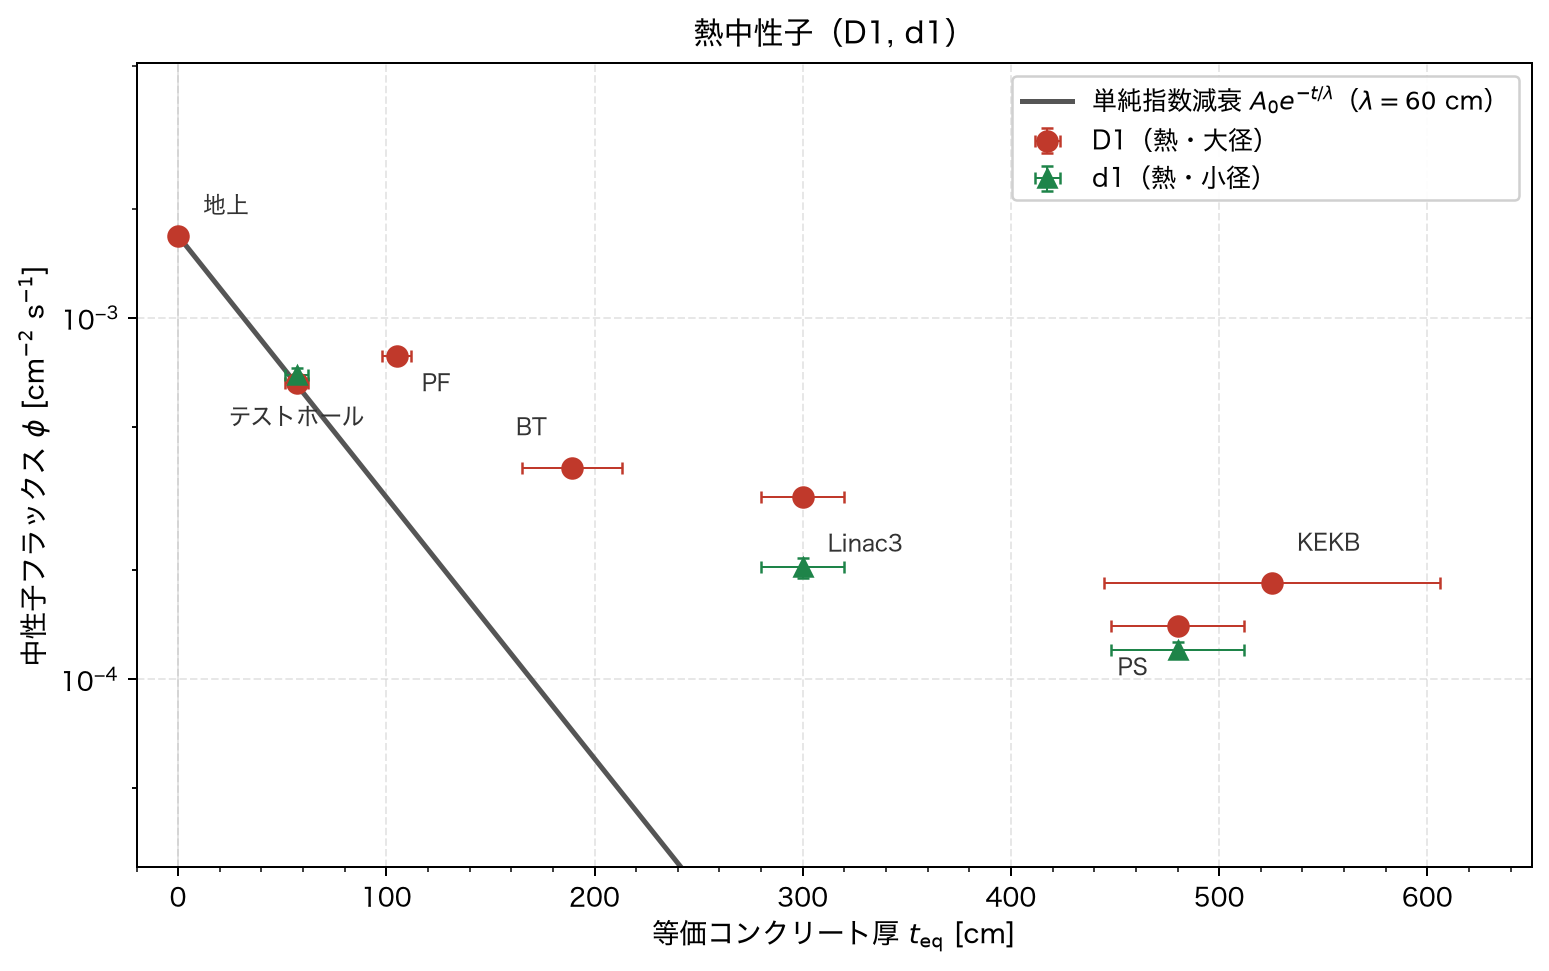
\includegraphics[width=0.86\linewidth]{figures/fig04_thermal_abs.png}\\[4pt]
  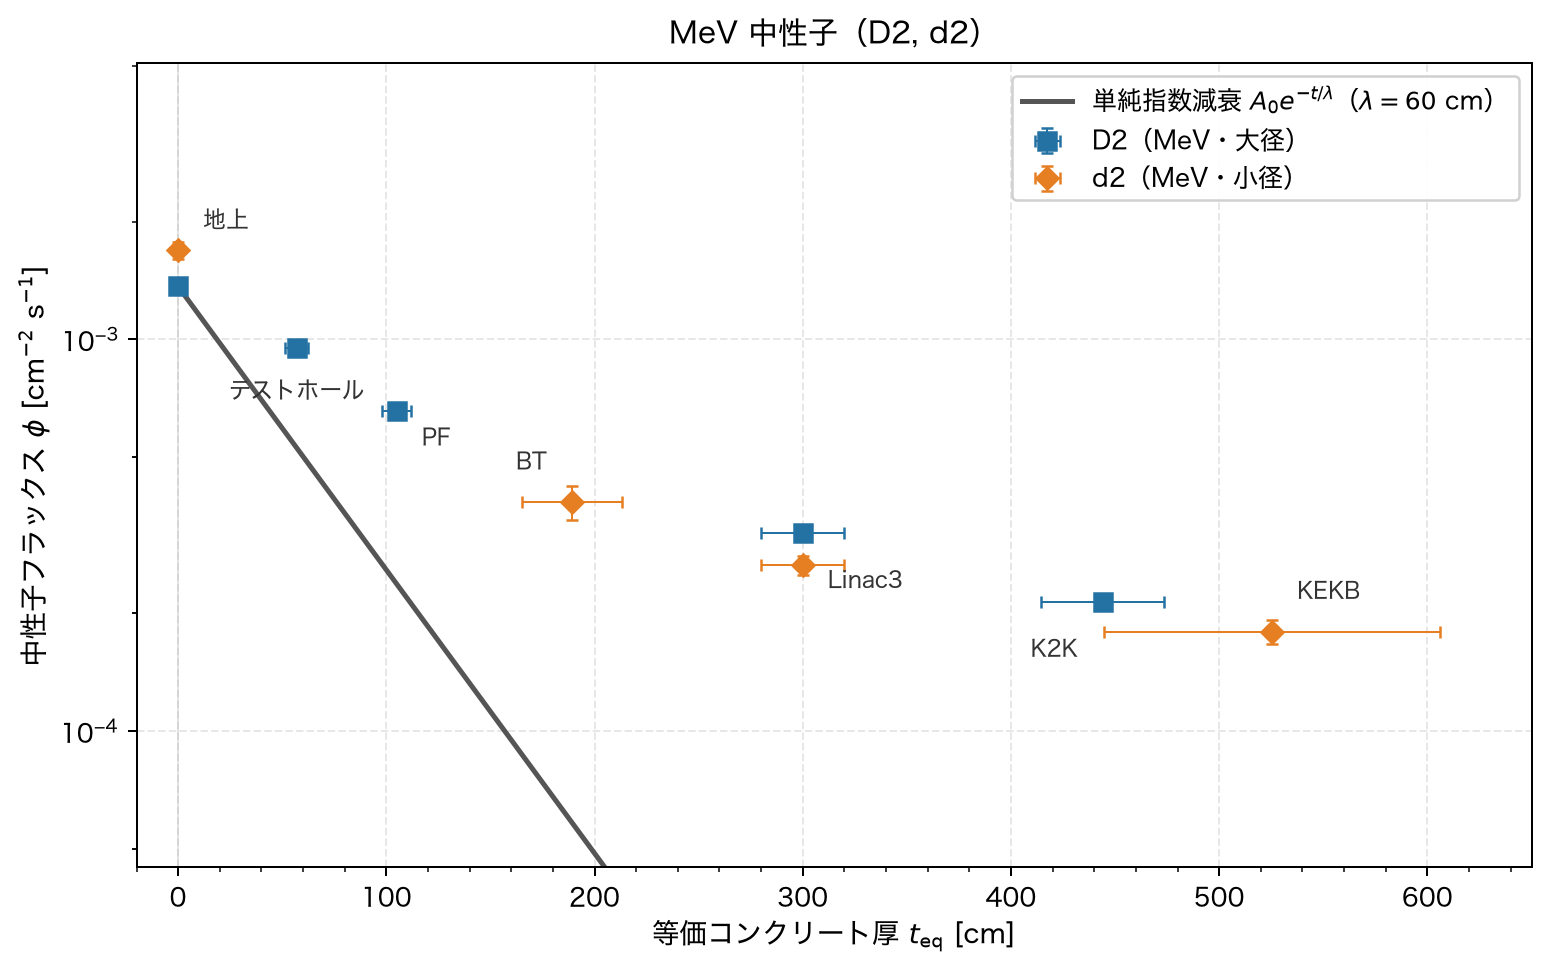
\includegraphics[width=0.86\linewidth]{figures/fig05_mev_abs.png}
  \caption{等価コンクリート厚に対する絶対フラックス。上：熱中性子（D1，d1），下：MeV 中性子（D2，d2）。
  縦の誤差棒は統計誤差，横の誤差棒は $\teq$ の系統誤差。
  灰色の実線は地上の実測値から引いた単純指数減衰（$\lambda=60$\,cm，式\eqref{eq:simple}）。}
  \label{fig:abs}
\end{figure}

\begin{figure}[htbp]
  \centering
  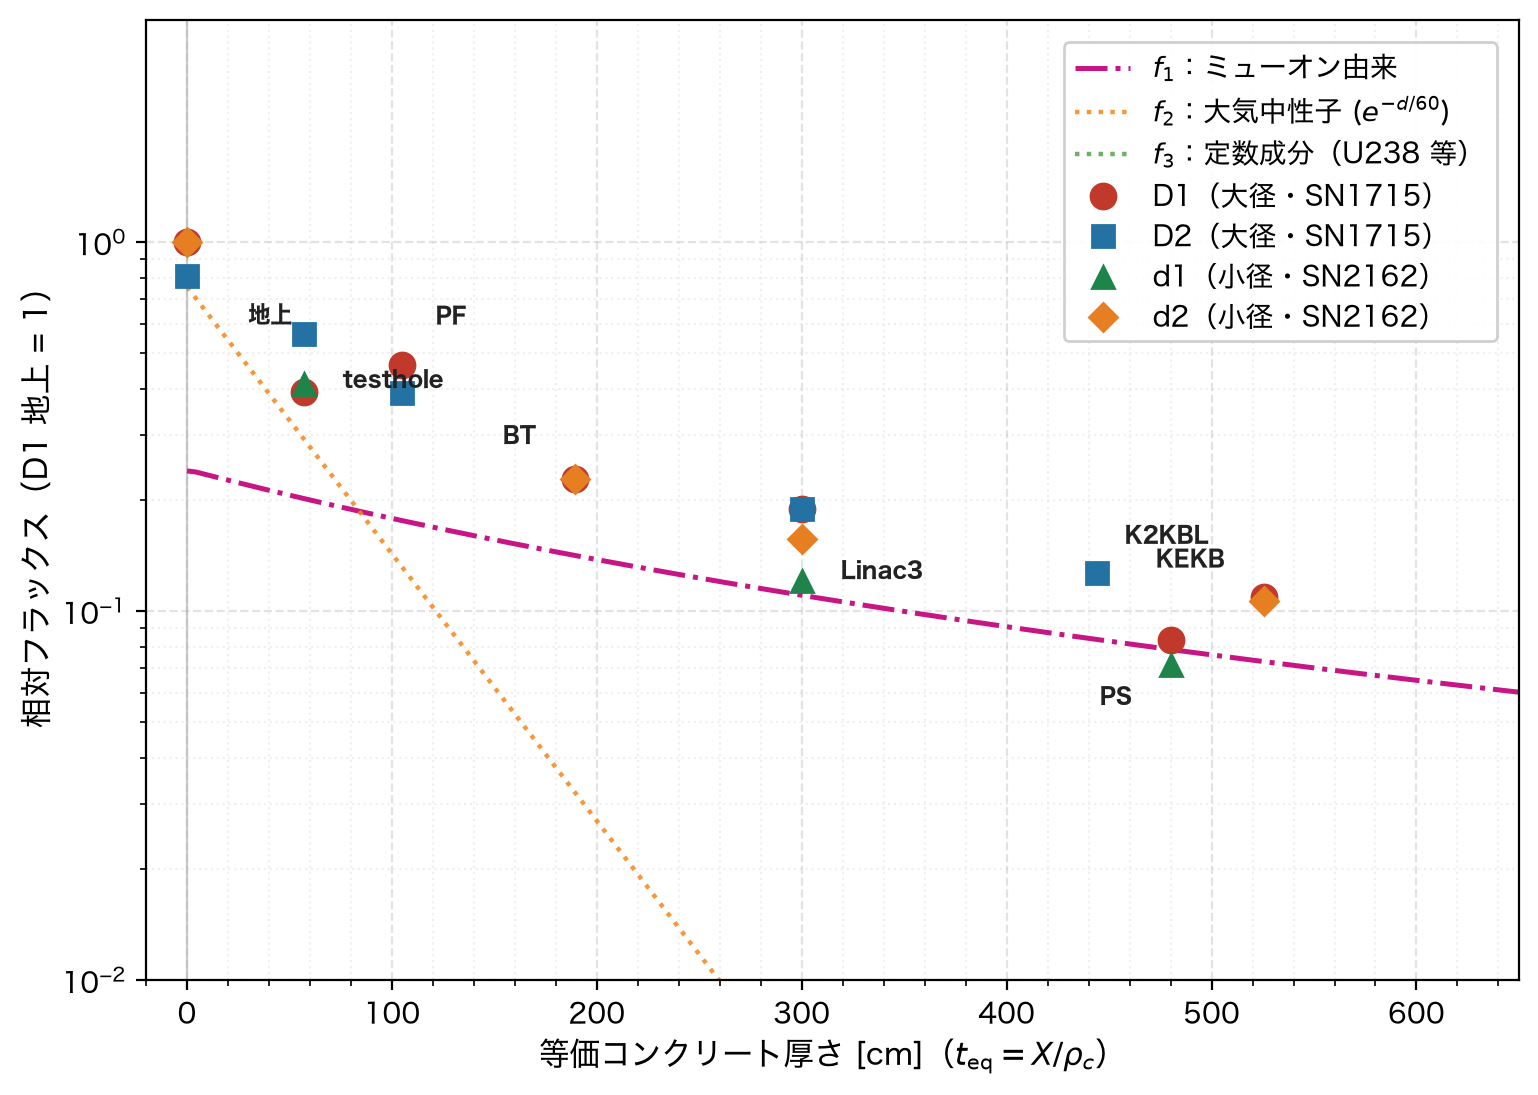
\includegraphics[width=0.78\linewidth]{figures/fig06_relative.png}
  \caption{4台の検出器の相対フラックス（D1 地上 $=1$ に規格化した絶対フラックス）。}
  \label{fig:rel}
\end{figure}

\subsection{単純指数減衰の予測との比較}

地上の実測値 $A_0$ に式\eqref{eq:simple}を適用した予測と実測の比を表\ref{tab:oldratio}に示す。
$\lambda_c=60$\,cm としても，実測は PF で約 3 倍，Linac3 で約 30 倍，KEKB で約 700 倍大きい。
教材値 $\lambda_c=39.2$\,cm では KEKB で約 $7\times10^{4}$ 倍に達する。
すなわち，\textbf{地下の中性子フラックスは，昨年度の結果から素直に想定される単純指数減衰では説明できず，深部（$\teq\ge300$\,cm）では予測と 1--3 桁ずれる}。

\begin{table}[htbp]
  \centering
  \caption{実測と単純指数減衰予測の比（$A_0$：熱は D1 地上，MeV は D2 地上）}
  \label{tab:oldratio}
  \begin{tabular}{lcrrrr}
    \toprule
    & & & & \multicolumn{2}{c}{実測/予測} \\
    \cmidrule(lr){5-6}
    地点 & 検出器 & $\teq$ [cm] & 地上比 $\phi/A_0$ & $\lambda=60$\,cm & $\lambda=39.2$\,cm \\
    \midrule
    テストホール & D1 & 57  & 0.391 & 1.0 & 1.7 \\
    PF          & D1 & 105 & 0.463 & 2.7 & 6.8 \\
    PF          & D2 & 105 & 0.482 & 2.8 & 7.0 \\
    放射線棟 BT  & D1 & 189 & 0.228 & 5.3 & 28 \\
    Linac3      & D1 & 300 & 0.189 & 28  & 400 \\
    Linac3      & D2 & 300 & 0.234 & 35  & 490 \\
    PS          & D1 & 480 & 0.083 & 250 & $1.7\times10^{4}$ \\
    KEKB        & D1 & 525 & 0.109 & 690 & $7.2\times10^{4}$ \\
    KEKB        & d2 & 525 & 0.132 & 840 & $8.7\times10^{4}$ \\
    \bottomrule
  \end{tabular}
\end{table}

\subsection{検出器間の整合性}
\label{sec:det}

同一地点で同時に測定した大径管と小径管のフラックス比を表\ref{tab:detratio}に示す。
テストホール（D1/d1）で 5\%，管理棟2階（D1/d1）で 15\%，PS（D1/d1）で 17\%，Linac3（D2/d2）で 21\% の範囲で一致した。
Linac3 の D1/d1 は 1.57 とやや大きい。
地上の D2/d2 は 0.81 である。d2 は地上で，D2 は Linac で D1 に合わせて較正したので，
これは「Linac でそろえた D2 と D1 の比が，地上では約 20\% 変わる」ことを意味し，PE 付き管の応答比が地点のスペクトルによって変わる程度の目安になる（\ref{sec:sys}節）。

\begin{table}[htbp]
  \centering
  \caption{同一地点での大径/小径のフラックス比}
  \label{tab:detratio}
  \begin{tabular}{llrr}
    \toprule
    地点 & 組 & 比 & $|\log_{10}(\text{比})|$ \\
    \midrule
    テストホール & D1/d1 & 0.95 & 0.023 \\
    管理棟2階 & D1/d1 & 1.15 & 0.060 \\
    PS & D1/d1 & 1.17 & 0.067 \\
    Linac3 & D2/d2 & 1.21 & 0.081 \\
    地上 & D2/d2 & 0.81 & 0.093 \\
    Linac3 & D1/d1 & 1.57 & 0.195 \\
    \bottomrule
  \end{tabular}
\end{table}

\subsection{昨年度との比較}

昨年度の裸管（今年度の d1 と同型の管）との比較を表\ref{tab:compare}に示す。
屋外（地上）の熱中性子フラックスは，昨年度 $1.70\times10^{-3}$，今年度 D1 で $1.69\times10^{-3}\,\flux$ と数値はよく近い。
ただし，この一致を較正の検証とみなすことはできない。
昨年度は黒鉛パイルでの実測で較正しているのに対し，今年度はメーカー感度を用いており，
今年度もパイルの直接測定を基準にするとフラックスは約 1.47 倍になる（\ref{sec:sys}節）。
また D1 の値は解析窓の選び方でも変わり，壁効果窓（191--764\,keV）で求めると $1.32\times10^{-3}\,\flux$ と約 22\% 小さい。
同じ型の d1 どうしで比べられる管理棟2階では，今年度の d1 は昨年度の 0.81 倍である。
したがって，昨年度と今年度の絶対値は，較正方法の違いによる数十\% の不確かさの範囲で整合している，というのが正確である。
屋内/屋外の比は同じ検出器の比で実効面積が約分されるのでこの不確かさを受けにくく，昨年度（管理棟2階/屋外）1.30--1.32 に対し今年度 1.23（壁効果窓でも 1.20）で，建物内の方がフラックスが高いという傾向を再現した。
これは建物の床・壁で減速・散乱された中性子（アルベド）が加わるためと考えられる。
管理棟1階/2階の比は昨年度 0.82，今年度 0.72 である。

\begin{table}[htbp]
  \centering
  \caption{昨年度（裸管）と今年度の熱中性子フラックスの比較 [$\flux$]}
  \label{tab:compare}
  \begin{tabular}{lrrrr}
    \toprule
    地点 & 昨年度 & 今年度 D1 & 今年度 d1 & 今年度 D1/昨年度 \\
    \midrule
    屋外（地上） & $1.70\times10^{-3}$ & $1.69\times10^{-3}$ & --- & 0.99 \\
    管理棟2階 & $2.21$--$2.25\times10^{-3}$ & $2.08\times10^{-3}$ & $1.81\times10^{-3}$ & 0.93 \\
    管理棟1階 & $1.83\times10^{-3}$ & $1.49\times10^{-3}$ & --- & 0.82 \\
    \bottomrule
  \end{tabular}
\end{table}

%======================================================================
\section{考察}
%======================================================================

\subsection{中性子の発生源の候補}
\label{sec:source}

単純指数減衰の予測が深部で合わなかったことから，測定場所の中性子は，大気中で作られて地表から入ってくる宇宙線中性子だけではないと考えた。
まず，加速器施設の地下で測定したので，加速器のビームに由来する中性子が候補になりうる。
しかし測定期間中（夏季停止期間）は全加速器が運転しておらず，ビームが物質に当たって中性子を作ることはなかったので，これは除外できる。
停止中も加速器の部材の残留放射能から $\gamma$ 線は出るが，そのエネルギーは数 MeV 以下で，
コンクリートの主な元素（O，Si，Ca，Al）の光核反応のしきい値（約 13--17\,MeV）に届かないため，中性子源にはならない。
K2K で低チャンネルの計数率が他地点の約10倍と高かった（\ref{sec:quality}節）のは，この $\gamma$ 線による可能性がある（未検証）。
$\gamma$ 線が \He 管に落とすエネルギーは小さく主に低チャンネルに現れるので，764\,keV のピーク領域への直接の影響は小さいが，部分補正の不確かさは大きくなる。

これを除いたうえで，地下で中性子を作りうるものとして，次の2つを候補に挙げた。

1つ目は大地（コンクリート・土）そのものに由来する中性子である。
コンクリートや土に含まれるウラン・トリウムは自発核分裂で中性子を出し，崩壊で出る $\alpha$ 線は軽い原子核と $(\alpha,n)$ 反応を起こす\cite{Wulandari2004}。
これらは宇宙線と関係がないので，深さにほとんど依らない一定の成分になる。
なお，検出器自身の $\alpha$ 汚染による計数は，スペクトルにそれらしい構造が目立って見えないことから主な原因ではないと判断した。

2つ目は，宇宙線のうち地下まで届く成分が，検出器のまわりの物質の中で新たに中性子を作る過程である。
こちらは地下に届く粒子の量に比例するので，深さとともにゆっくり減ると期待される。

\subsection{地下まで届く宇宙線成分}

地表に届く宇宙線の各成分について，地下まで届くか，届いた先で中性子を作れるかを表\ref{tab:particles}にまとめた。
陽子・$\pi$ 中間子・電子は，コンクリート中ですぐにエネルギーを失うか崩壊するため，数 m の遮蔽の下にはほとんど残らない。
ニュートリノは地下まで届くが，物質とほとんど反応しない。
$\gamma$ 線は光核反応で中性子を出せるが，コンクリートの主な元素ではしきい値が約 13--17\,MeV と高く，断面積が大きいのは巨大共鳴（約 15--25\,MeV）付近に限られ，その値も小さい。

残るミューオンは透過力が高い。PHITS の計算でも，コンクリート 2.5\,m の下で地表の約 72\% が残っていた（\ref{sec:phits}節）。
LHC-FASER 実験でも，衝突点から約 100\,m の岩盤・コンクリートを通り抜けてくるのはミューオンとニュートリノがほとんどであり，
ミューオンがまわりの物質と反応して作る二次粒子が背景事象になることが報告されている\cite{FASER2026}。

ミューオンが中性子を作る過程には，高エネルギーのミューオンが原子核を壊す核破砕や，ミューオンが起こすシャワー中の光核反応のほかに，
物質中で止まった負ミューオンが原子核に捕獲される反応
\begin{equation}
  \mu^- + p \;\to\; n + \nu_\mu
\end{equation}
がある。負ミューオンはまずミューオン原子を作り，その一部が原子核内の陽子に捕獲される。
捕獲されたあとの原子核は，励起エネルギー 10--20\,MeV を中心に，最大 100\,MeV 程度まで励起され，主に中性子を放出して脱励起する\cite{Mizuno2025,MizunoJPS2026}。
止まった負ミューオンのうち捕獲に至る割合は原子番号とともに大きくなり，コンクリートに最も多い O では約 18\%\cite{Suzuki1987}，
Si と Al ではそれぞれ約 66\%，61\% である。
捕獲後は荷電粒子を伴わない中性子放出が支配的である（${}^{27}$Al では中性子1個の放出だけで 70\% 以上）\cite{Mizuno2025}。
このように，地下まで届いたミューオンは，止まる前にも止まったあとにも中性子を作ることができる。

\begin{table}[htbp]
  \centering
  \caption{宇宙線の各成分と地下での振る舞い}
  \label{tab:particles}
  \small
  \begin{tabular}{lp{8.4cm}cc}
    \toprule
    成分 & 地下での振る舞い & 地下に到達 & 中性子源 \\
    \midrule
    ミューオン ($\mu^\pm$) & 透過力が高く，地下まで到達して中性子を生成する反応を起こす & ○ & 主要 \\
    $\gamma$ 線 & 地表の $\gamma$ 線は遮蔽で吸収されるが，地下でもミューオンの反応で二次的に生じる。光核反応で中性子を生成できるが，反応断面積が小さい & ○（二次） & 小さい \\
    陽子 & 地下で急速にエネルギーを失うので残りにくい & × & --- \\
    $\pi$ 中間子 & 強い相互作用と短い寿命のため地下まで残りにくい & × & --- \\
    電子・陽電子 & 地下で急速にエネルギーを失うので残りにくい & × & --- \\
    ニュートリノ & 透過力は高いが，相互作用確率が極端に小さく反応を起こさない & ○ & 無視できる \\
    \bottomrule
  \end{tabular}
\end{table}

\subsection{文献に見るミューオン起源の中性子}

深さによって中性子の作られ方がどう変わるかを，Fabryka-Martin\cite{FabrykaMartin1988}の見積もりで確認した（図\ref{fig:fm}）。
遮蔽の薄いところでは宇宙線中性子による生成（蒸発中性子）が大部分を占めるが，厚さとともに急に減り，数 m を超えると負ミューオン捕獲による生成の方が大きくなる。
さらに数十 m より深いところでは，$(\alpha,n)$ 反応と自発核分裂による一定の成分だけが残る。
今回の測定範囲（$\teq=0.6$--$5.3$\,m）は，ちょうど中性子の主な作られ方が宇宙線中性子からミューオンへ移り変わる深さにあたる。
ただし，図の縦軸は物質 1\,kg あたりの中性子の生成率であり，検出器の位置でのフラックスとは直接比べられないので，ここでは傾向を見るためだけに用いた。

\begin{figure}[htbp]
  \centering
  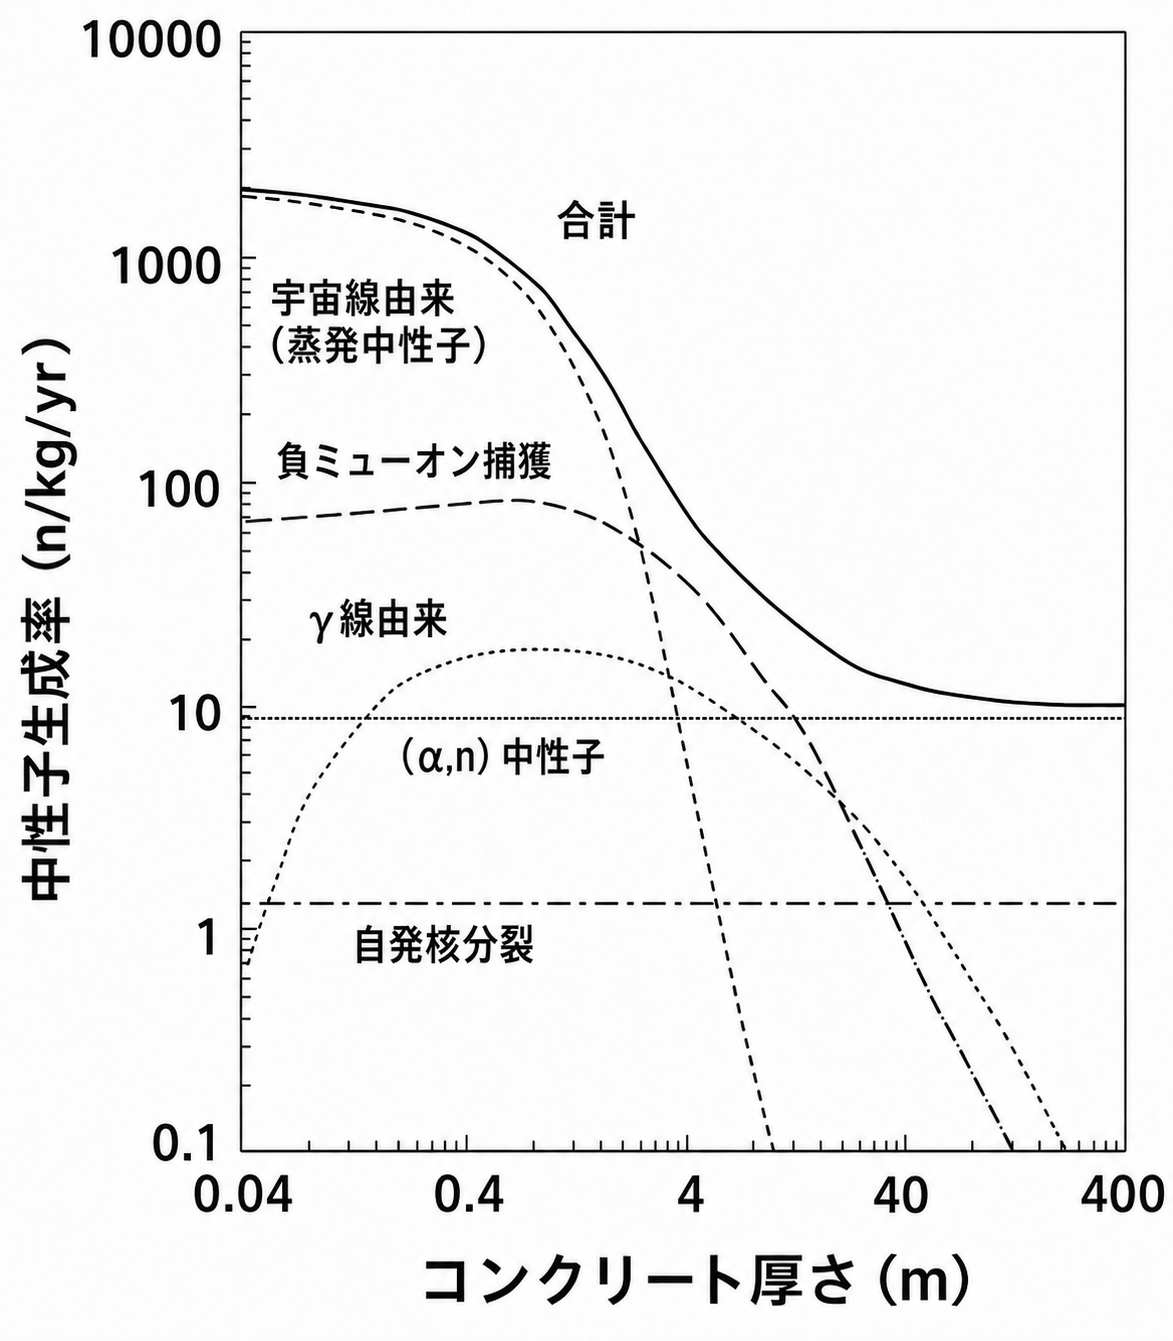
\includegraphics[width=0.55\linewidth]{figures/fig09_fabryka_martin.png}
  \caption{遮蔽の厚さに対する中性子生成率の内訳。文献\cite{FabrykaMartin1988}の図をもとに作成（軸・凡例を和訳）。}
  \label{fig:fm}
\end{figure}

\subsection{PHITS で見たミューオンによる中性子生成}

ミューオンが地下で中性子を作る様子を PHITS\cite{PHITS}で確認した（図\ref{fig:phitsmu}）。
コンクリート（黄）の中にトンネル（青）がある体系に上からミューオンを入射すると，コンクリートを通り抜けるミューオン（水色・白の線）に沿って中性子（赤）が生じ，
トンネルの周囲やトンネル内にも中性子が現れる。
生成過程ごとの寄与を定量的に切り分けた計算は\ref{sec:phitscomp}節で述べる。

\begin{figure}[htbp]
  \centering
  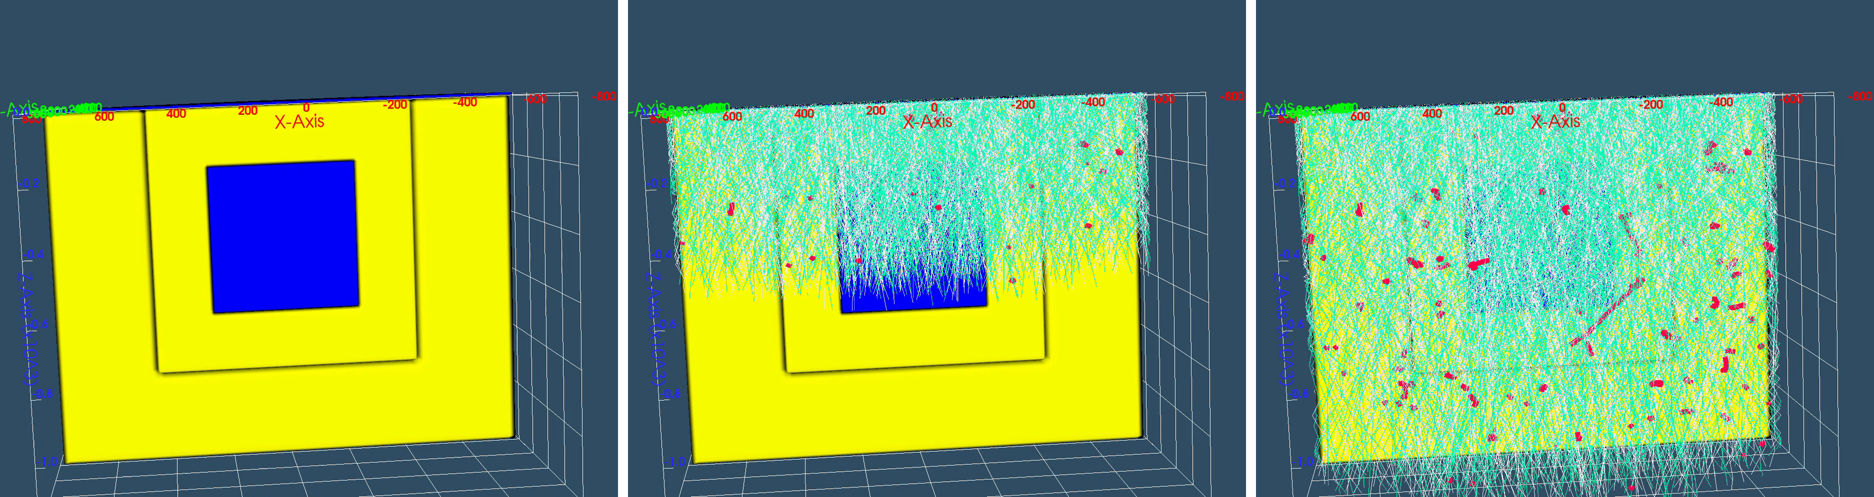
\includegraphics[width=\linewidth]{figures/fig10_phits_muon.png}
  \caption{PHITS で計算したミューオンによる中性子生成の様子（最終発表で示した動画から3コマを抜き出した）。
  左から順に入射したミューオンの数が増えていく。黄はコンクリート，青はトンネル，水色・白の線はミューオン，赤は中性子。}
  \label{fig:phitsmu}
\end{figure}

\subsection{ミューオン起源中性子の定式化}

深さ $d$ でのミューオン起源中性子の生成は，文献\cite{MeiHime2006,Wang2001}に従い
\begin{equation}
  N(d) = I_\mu(d)\times Y_n(\bar{E}_\mu)\times\Delta x
  \label{eq:Nd}
\end{equation}
と書ける。ここで $I_\mu(d)$ は深さ $d$ でのミューオン強度，
$Y_n$ は1個のミューオンが単位質量厚さあたりに作る中性子数（収量），$\bar{E}_\mu$ は深さ $d$ でのミューオンの平均エネルギー，
$\Delta x$ は中性子の生成に寄与する層の質量厚さである。

本研究では，深さを水当量 $d=\rho_c\teq/100$ [m.w.e.] で表し，各因子を次のべき型で近似した。
\begin{align}
  I_\mu(d) &= I_0\left(1+\frac{d}{d_0}\right)^{-\gamma},
  & I_0 &= 100\ \mathrm{m^{-2}\,s^{-1}},\ d_0=11.5\ \mathrm{m.w.e.},\ \gamma=2.2, \\
  \bar{E}_\mu(d) &= E_0\left(1+\frac{d}{d_0}\right)^{\alpha},
  & E_0 &= 4\ \mathrm{GeV},\ \alpha=0.73, \\
  Y_n(\bar{E}_\mu) &= \sum_i a\,(a_i)^{\beta}\,\bar{E}_\mu^{\,\alpha},
  & a &= 4.0\times10^{-6}\ \mathrm{n\,\mu^{-1}\,(g\,cm^{-2})^{-1}\,GeV^{-\alpha}}.
\end{align}
$Y_n\propto\bar{E}_\mu^{0.73}$ というエネルギー依存は Wang ら\cite{Wang2001}の収量式 $Y_n\propto\bar{E}_\mu^{0.74}$ に，
標的の質量数への依存 $(a_i)^{\beta}$ は Mei と Hime\cite{MeiHime2006}の $A^{0.95}$ 型の依存に対応する。
$a_i$ はコンクリートの組成ごとの寄与を表すために導入した係数の組で，MeV 中性子に対しては6成分の組 $(13.2, 8.4, 3.2, 1.35, 1.68, 0.01)$ と $\beta=0.90$ を用いた。
ただし個々の $a_i$ は元素ごとの測定値や文献値から決めたものではなく，後述のとおり実測に合わせて調整した値である。
$I_\mu$ と $\bar{E}_\mu$ のべき型も，地表の典型値（強度約 $100\,\mathrm{m^{-2}\,s^{-1}}$，平均エネルギー約 4\,GeV）を端点として浅い地下の深さ依存を表すように選んだ経験的な近似であり，$d_0$，$\gamma$，$\alpha$ は特定の文献の値ではない。
生成層の厚さは $\Delta\bar{x}=230\,\gcm$（コンクリート 1\,m 相当）とした。
なお，$\bar{E}_\mu$ の深さ依存の指数と $Y_n$ のエネルギー依存の指数は物理的には別の量であるが，ここでは両者に同じ値 $\alpha=0.73$ を用いた。

ただし，Wang らや Mei と Hime の収量式は，深い地下（数百 m.w.e. 以上）での\textbf{高速ミューオン}による中性子生成を表すものであり，
止まった負ミューオンの捕獲は含まない。捕獲による生成率はミューオンが止まる割合（$-dI_\mu/dX$ に比例）で決まり，$I_\mu\times Y_n$ の形にはならない。
今回の浅い深さでは後述のように捕獲が支配的と考えられるので（\ref{sec:phitscomp}節），式\eqref{eq:Nd}は捕獲の寄与も係数に押し込んだ経験的な式として扱う。

\subsection{多成分モデル}
\label{sec:model}

MeV 中性子のフラックスを次の3成分の和で表した。
\begin{equation}
  \phi(\teq) = f_1(\teq) + f_2(\teq) + f_3
  \label{eq:model}
\end{equation}
$f_1$ はミューオン起源の中性子で，式\eqref{eq:Nd}を深さ $d\pm0.1$\,m.w.e. の範囲（地表付近では $0$ から $d+0.1$\,m.w.e. まで）で平均した値である。
$f_2 = F_0\,e^{-\teq/60\,\mathrm{cm}}$（$F_0=1.189\times10^{-3}\,\flux$）は大気由来の中性子の指数減衰，
$f_3=3.88\times10^{-6}\,\flux$ は大地に由来する深さに依らない成分である。
関数形は文献に基づくが，係数（$a_i$，$\beta$，$\Delta\bar{x}$，$F_0$，$f_3$）は実測との一致を見ながら手で調整した値であり，統計的なフィットではない。
したがって以下の一致の良さは，モデルが独立に予測した結果ではなく，この関数形で実測の深さ依存を表せることを示すものである。

モデルと実測の比較を図\ref{fig:theory}に，各点の実測/モデル比を表\ref{tab:modelratio}に示す。
$\teq\approx50$\,cm より浅いところでは $f_2$ が，それより深いところでは $f_1$ が大きく，$\teq=300$\,cm ではモデルの 96\% を $f_1$ が占める。
$f_3$ の寄与は今回の深さの範囲では 3\% 以下である。
ただしこのモデルでは地上でも MeV 中性子の 32\% を $f_1$ が占め，PHITS の計算（2\%，\ref{sec:phitscomp}節）より1桁以上大きい。
浅いところの $f_1$ は過大で，その分を $f_2$ の係数が小さめに吸収していると考えられるので，モデルの成分の内訳が意味をもつのは深部に限られる。
8点の実測/モデル比は 0.77--1.16 で，対数残差の二乗平均平方根（RMS）は 0.048\,dex（倍率で約 1.12 倍）となった。
同じ8点で単純指数減衰（$\lambda=60$\,cm）と比べた場合の 1.57\,dex（約 37 倍）に比べると，ずれは大きく縮まった。
ただし係数は実測を見ながら手で合わせたものなので，この小さな RMS はモデルの予言力ではなく，関数形の表現力を示すにすぎない。
地下の MeV 中性子フラックスが深さに対して落ちきらないことは，ミューオンが地下で作る中性子を加えることで，オーダーとして説明できる。

熱中性子については，同じ形のモデルとの定量的な比較は行わなかった。
熱中性子のフラックスは，MeV 中性子がまわりの物質の水素などで減速される過程に強く依存し，トンネルの形や壁の含水量の影響を受けるが，
今回のモデルではその過程を扱えていないためである。
ただし，深部の熱中性子フラックスは MeV 中性子と同じように深さに対して落ちきらず（図\ref{fig:abs}），
同じ起源の中性子が周囲で熱化したものと考えれば定性的には矛盾しない（両者の絶対値がそろって見えるのは D2 の較正による）。

\begin{figure}[htbp]
  \centering
  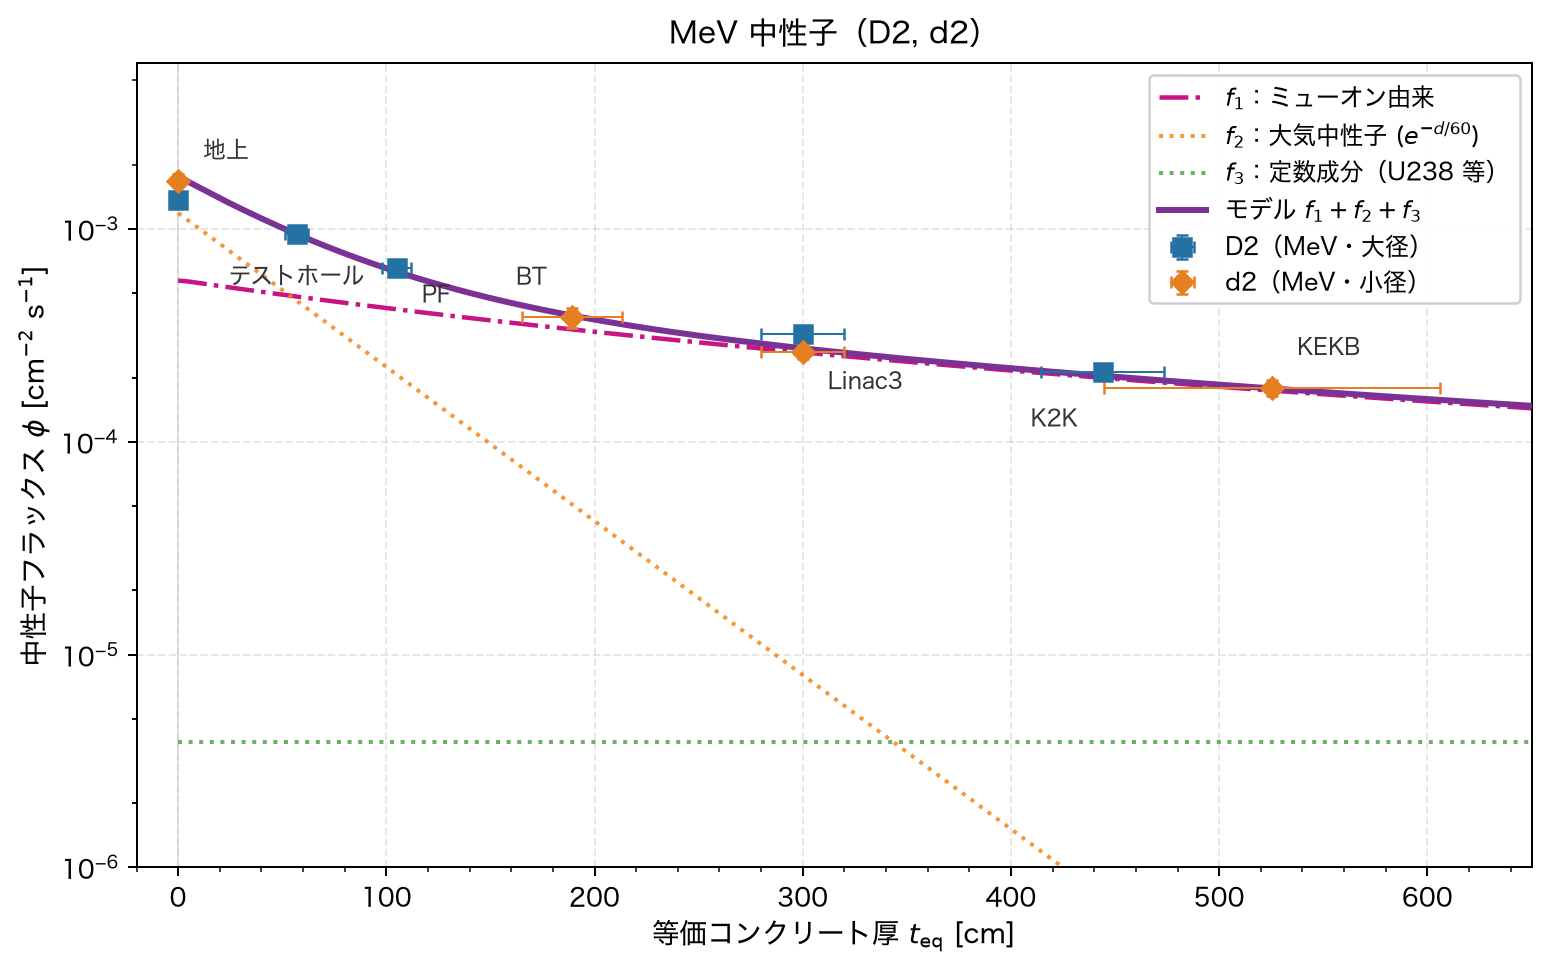
\includegraphics[width=0.86\linewidth]{figures/fig08_mev_theory.png}
  \caption{MeV 中性子の多成分モデル（紫の実線 $f_1+f_2+f_3$）と実測の比較。
  縦の誤差棒は統計誤差と置き場所の系統誤差（4.75\%）の二乗和。}
  \label{fig:theory}
\end{figure}

\begin{table}[htbp]
  \centering
  \caption{MeV 中性子の実測と多成分モデルの比，およびモデル中のミューオン起源成分 $f_1$ の割合}
  \label{tab:modelratio}
  \small
  \begin{tabular}{lcrrrr}
    \toprule
    地点 & 検出器 & $\teq$ [cm] & 実測 $\phi$ [$\flux$] & 実測/モデル & $f_1$ の割合 \\
    \midrule
    地上 & D2 & 0 & $1.37\times10^{-3}$ & 0.77 & 0.32 \\
    地上 & d2 & 0 & $1.69\times10^{-3}$ & 0.96 & 0.32 \\
    PF & D2 & 105 & $6.58\times10^{-4}$ & 1.04 & 0.67 \\
    放射線棟 BT & d2 & 189 & $3.84\times10^{-4}$ & 0.98 & 0.86 \\
    Linac3 & D2 & 300 & $3.20\times10^{-4}$ & 1.16 & 0.96 \\
    Linac3 & d2 & 300 & $2.65\times10^{-4}$ & 0.96 & 0.96 \\
    K2K & D2 & 444 & $2.14\times10^{-4}$ & 1.05 & 0.98 \\
    KEKB & d2 & 525 & $1.80\times10^{-4}$ & 1.01 & 0.98 \\
    \bottomrule
  \end{tabular}\\[2pt]
  \footnotesize D2 テストホール（D1 との重複データ，比 1.00）は表から省いた。
\end{table}

\subsection{PHITS シミュレーション}
\label{sec:phits}

本研究の PHITS\cite{PHITS}の計算にはバージョン 3.36（Web 版）を用いた。
ただし断面のフラックス分布の図（図\ref{fig:detmap}，\ref{fig:sitemap}）だけは，同じ体系をバージョン 3.35（ローカル版）で計算した。

\paragraph{地上の絶対値と建屋の効果}
PHITS の宇宙線線源（PARMA/EXPACS\cite{Sato2015}，KEK つくばの緯度・経度・標高）を用い，
入射器棟（Linac）の断面を図面から再現した3次元モデルで各位置のフラックスを計算した（5000 ヒストリー）。
開空の地上 1.3\,m での中性子の全エネルギー積分フラックスは $(3.68\pm0.46)\times10^{-3}\,\flux$ で，
昨年度の3領域合計（約 $3.4\times10^{-3}$）と同程度であった。
建屋内（クライストロンギャラリー）では熱中性子が開空の約 8.7 倍に増えた。
屋内で増えるという向きは実測と同じだが，実測の増え方（管理棟で約 1.2 倍）よりはるかに大きく，
建屋の模型（壁の材質・含水量や検出器の位置）に強く依存すると考えられるので，定量的な比較には使えない。
一方，コンクリート 2.5\,m 下のトンネルでは中性子は $8.6\times10^{-5}\,\flux$（統計誤差 67\%）まで減るが，
ミューオンは開空の 72\% が残っていた。

\paragraph{1次元スラブモデルでの見積もり}
天井スラブの厚さだけを変えた1次元モデルでは，PF（$\teq=105$\,cm）で
\He 管のエネルギー付与の地上比が $10^{-5}$ 程度となった。
しかしこれは管の体積が小さくエネルギー付与の統計がほぼゼロだったためで，同じ計算で管の位置の中性子フラックスを見ると地上比は 0.46 であり，実測（約 0.48）に近かった。
一方，別の検出器配置で行った同じ計算では 0.03 となるなど計算ごとのばらつきが大きく，この計算からは結論を出せない。
そこで統計を確保した計算を改めて行った（\ref{sec:phitscomp}節）。

\paragraph{検出器の置き場所による系統誤差}
トンネル断面を模したモデルにミューオンと中性子を入射し，天井厚 2\,m のとき
検出器を壁に寄せた場合と通路の中央に置いた場合のフラックスを比較した。
壁寄りで $(4.745\pm0.069)\times10^{-4}$，中央で $(4.970\pm0.069)\times10^{-4}\,\flux$ となり，
差は $(2.25\pm0.98)\times10^{-5}\,\flux$（約 4.75\%）であった。
この値を置き場所による系統誤差として図\ref{fig:theory}の誤差棒に加えた。
この大きさは，多成分モデルと実測の差（RMS で約 12\%）と同程度である。

\subsection{PHITS による線源成分ごとの中性子深さ分布}
\label{sec:phitscomp}

\paragraph{計算の方法}
地表より下を一様なコンクリート（密度 2.3\,g\,cm$^{-3}$，水素 1.0\,wt\%）で満たした半無限の体系に，KEK つくばの宇宙線線源（PARMA）を入射し，
深さ 20\,cm ごとの中性子フラックスを求めた。
線源の粒子の種類を分けて，(i) 大気由来のハドロン（中性子と陽子），(ii) $\mu^-$，(iii) $\mu^+$ の3通りを計算した。
$\mu^+$ は原子核に捕獲されないので，$\mu^+$ による中性子は高速ミューオンによる核破砕・ミューオン核反応・シャワー中の光核反応だけで作られる。
これらの過程は電荷の符号にほとんど依らないため，地表での $\mu^-/\mu^+$ フラックス比を $R$（PARMA で 0.858）として
\begin{equation}
  \phi_{\mathrm{cap}} = \phi(\mu^-) - R\,\phi(\mu^+), \qquad \phi_{\mathrm{fast}} = (1+R)\,\phi(\mu^+)
\end{equation}
により，負ミューオン捕獲による成分 $\phi_{\mathrm{cap}}$ と高速ミューオンによる成分 $\phi_{\mathrm{fast}}$ を切り分けた。
ハドロンの計算では深さ 50\,cm ごとに重要度（importance）を 2 倍にして深部の統計を確保し，線源球の側面から地中へ直接入る非物理的な粒子は除いた。
Web 版 PHITS の実行時間の制限（1ジョブ3分）のため，乱数の種を変えた計 54 ジョブ（$\mu^-$ は約 $2\times10^4$ 個）を積算した。
実測との比較には，熱中性子では裸管の $1/v$ 応答に合わせて $\sqrt{0.0253\,\mathrm{eV}/E}$ で重み付けしたフラックスを，
MeV 中性子では 0.1--20\,MeV の中性子フラックスを用いた。

\paragraph{結果}
各成分の深さ分布を図\ref{fig:phitscomp}に，測定地点での値を表\ref{tab:phitscomp}に示す。
大気由来のハドロンによる成分は深さとともにほぼ指数関数的に減り，$\teq=105$--525\,cm での実効的な減衰長は約 80\,cm（$184\,\gcm$）であった。
これは $\lambda=60$\,cm より緩く，岩石中の宇宙線核種生成で用いられる $\Lambda\approx160\,\gcm$\cite{Gosse2001}に近い。
浅い地点（PF，BT）では実測/PHITS が熱中性子で 0.7，MeV 中性子で 1.1 と，絶対値が2倍以内で合っている。

一方，負ミューオン捕獲による成分は深さに対してゆっくりとしか減らず，$\teq\approx170$--180\,cm でハドロンによる成分を上回った（図\ref{fig:phitsfrac}左）。
$\teq\ge300$\,cm では中性子の 72--97\% がミューオン起源で，その大部分（全体の 66--93\%）が負ミューオン捕獲による。
高速ミューオンによる成分は捕獲による成分の数分の1以下であった。
PHITS の中では，コンクリート中で止まった $\mu^-$ の 42\% が原子核に捕獲され（残りは崩壊），
$\mu^-$ の計算全体で生じた中性子の数は捕獲1回あたり約 1.2 個であった（捕獲以外の過程による中性子も含む）。
この傾向は，\ref{sec:model}節のモデルで深部の大部分を $f_1$ が占めたことや，Fabryka-Martin の見積もり（図\ref{fig:fm}）と一致し，
深部の中性子が主に地下まで届いたミューオン，特に止まった負ミューオンの捕獲で作られるという解釈を支持する。

\begin{figure}[htbp]
  \centering
  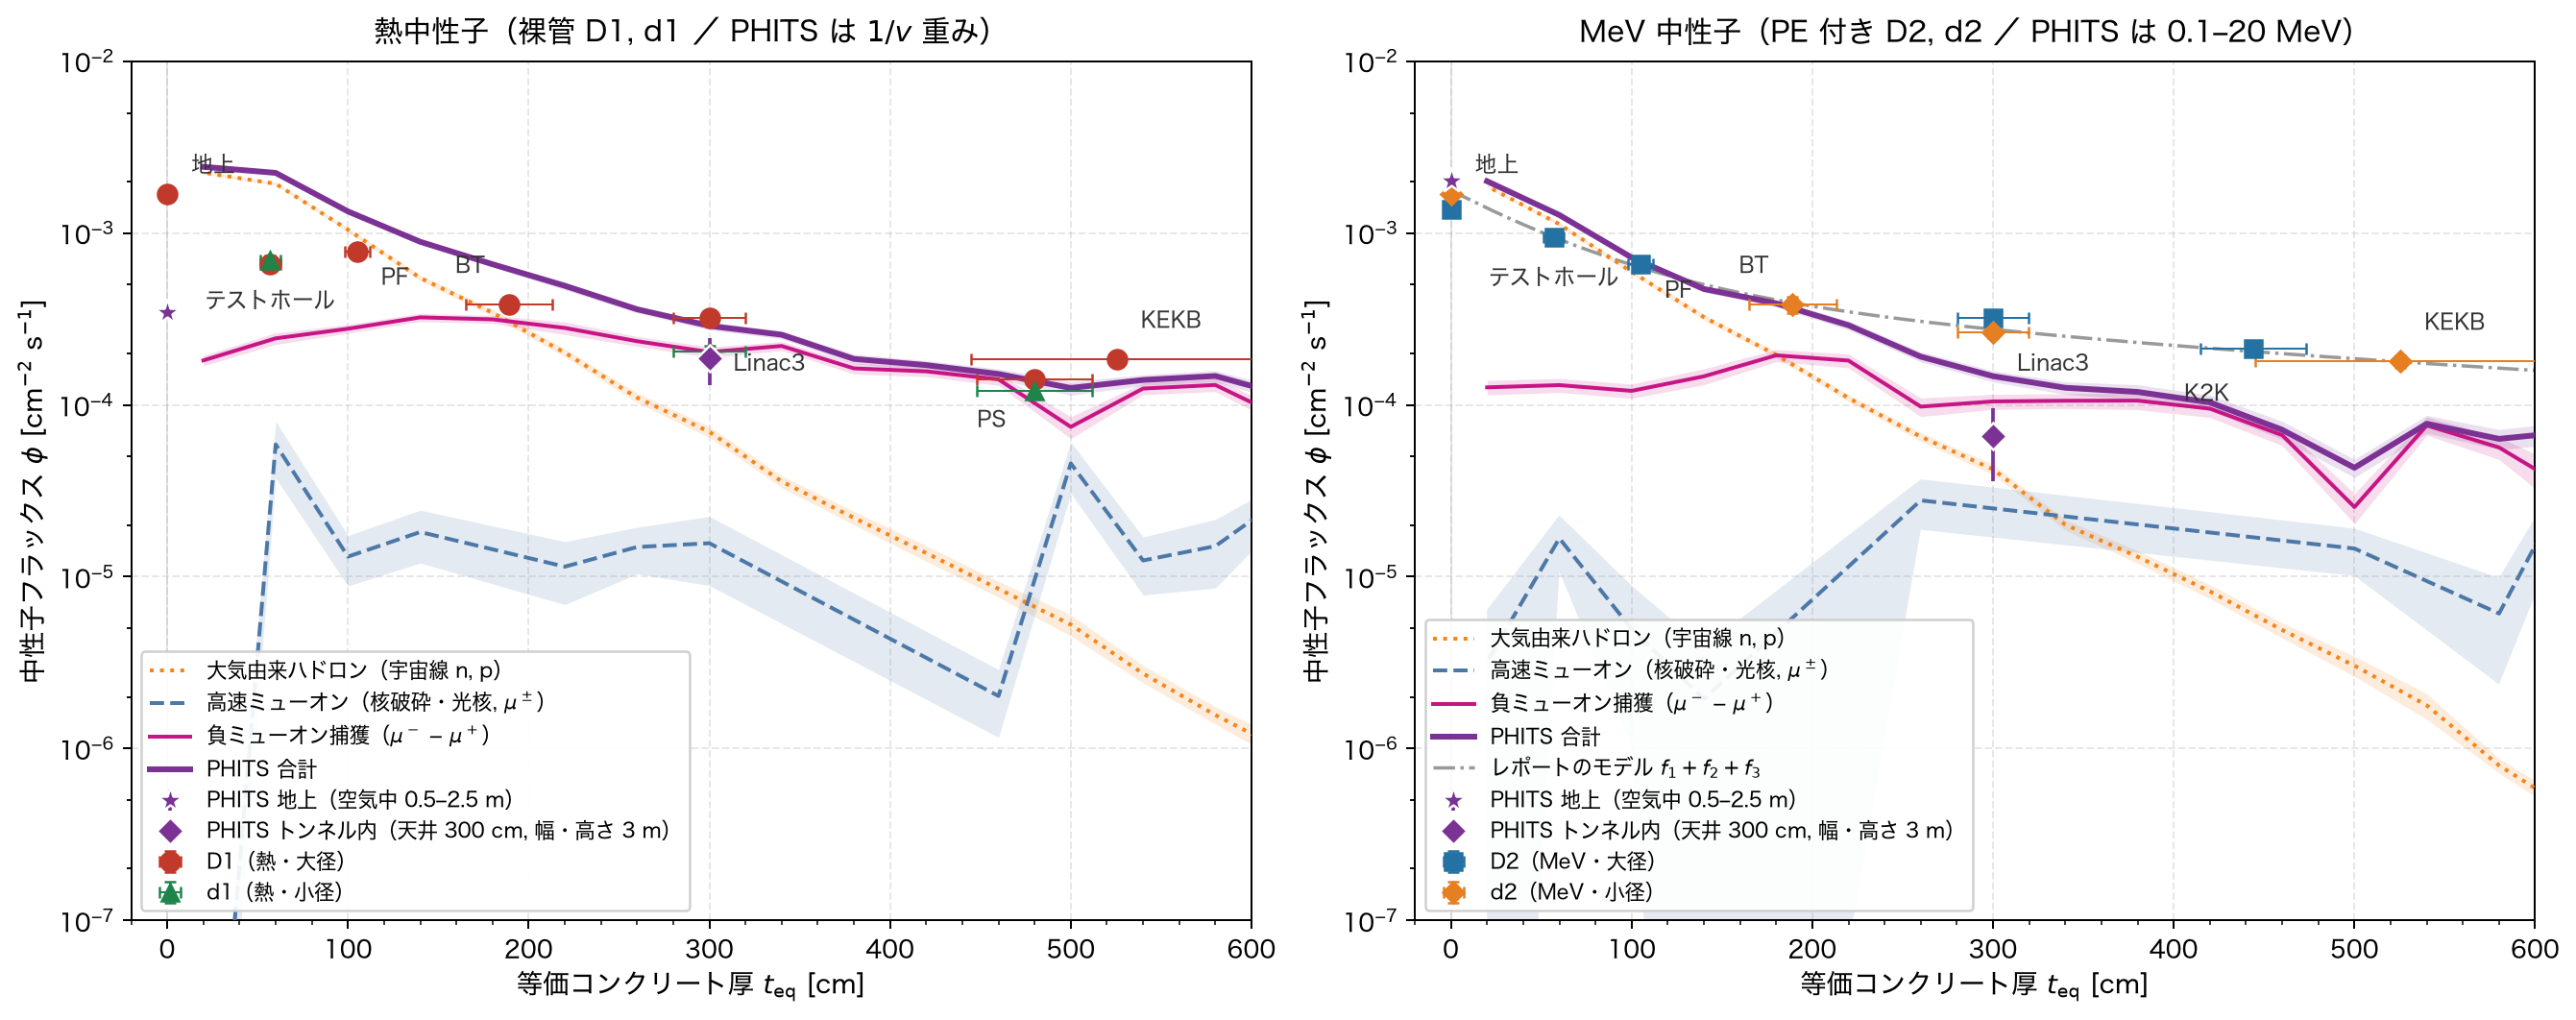
\includegraphics[width=\linewidth]{figures/fig11_phits_components.png}
  \caption{PHITS で計算した線源成分ごとの中性子フラックスの深さ分布と実測の比較。左：熱中性子（PHITS は $1/v$ 重み），右：MeV 中性子（PHITS は 0.1--20\,MeV）。
  橙：大気由来のハドロン，赤紫：負ミューオン捕獲（$\mu^-$ と $\mu^+$ の差），青破線：高速ミューオン，紫：合計。帯は統計誤差。
  星印は地上の空気中，菱形は天井厚 300\,cm のトンネル内の PHITS の値。右図の灰色の一点鎖線は\ref{sec:model}節のモデル。}
  \label{fig:phitscomp}
\end{figure}

\begin{table}[htbp]
  \centering
  \caption{測定地点での実測と PHITS（半無限コンクリート中，$\teq\pm40$\,cm の平均）の比較。フラックスの単位は $\flux$，
  「$\mu$ 起源」「うち捕獲」は PHITS 合計に占めるミューオン起源と負ミューオン捕獲の割合。}
  \label{tab:phitscomp}
  \small
  \setlength{\tabcolsep}{4.5pt}
  \begin{tabular}{llcrrrrrr}
    \toprule
    & 地点 & 検出器 & $\teq$ [cm] & 実測 & PHITS 合計 & 実測/PHITS & $\mu$ 起源 & うち捕獲 \\
    \midrule
    熱 & 地上 & D1 & 0 & $1.69\times10^{-3}$ & $3.48\times10^{-4}$ & 4.86 & 0.09 & 0.09 \\
       & テストホール & D1 & 57 & $6.61\times10^{-4}$ & $2.33\times10^{-3}$ & 0.28 & 0.10 & 0.09 \\
       & PF & D1 & 105 & $7.83\times10^{-4}$ & $1.11\times10^{-3}$ & 0.70 & 0.28 & 0.27 \\
       & 放射線棟 BT & D1 & 189 & $3.85\times10^{-4}$ & $5.75\times10^{-4}$ & 0.67 & 0.53 & 0.52 \\
       & Linac3 & D1 & 300 & $3.20\times10^{-4}$ & $3.01\times10^{-4}$ & 1.06 & 0.76 & 0.73 \\
       & PS & D1 & 480 & $1.41\times10^{-4}$ & $1.38\times10^{-4}$ & 1.02 & 0.95 & 0.78 \\
       & KEKB & D1 & 525 & $1.84\times10^{-4}$ & $1.32\times10^{-4}$ & 1.39 & 0.97 & 0.75 \\
    \midrule
    MeV & 地上 & D2 & 0 & $1.37\times10^{-3}$ & $2.03\times10^{-3}$ & 0.67 & 0.02 & 0.02 \\
        & PF & D2 & 105 & $6.58\times10^{-4}$ & $5.96\times10^{-4}$ & 1.10 & 0.23 & 0.22 \\
        & 放射線棟 BT & d2 & 189 & $3.84\times10^{-4}$ & $3.40\times10^{-4}$ & 1.13 & 0.55 & 0.55 \\
        & Linac3 & D2 & 300 & $3.20\times10^{-4}$ & $1.54\times10^{-4}$ & 2.07 & 0.72 & 0.66 \\
        & K2K & D2 & 444 & $2.14\times10^{-4}$ & $8.74\times10^{-5}$ & 2.44 & 0.93 & 0.93 \\
        & KEKB & d2 & 525 & $1.80\times10^{-4}$ & $6.03\times10^{-5}$ & 2.97 & 0.96 & 0.84 \\
    \bottomrule
  \end{tabular}\\[2pt]
  \footnotesize 地上の PHITS は空気中（地表から 0.5--2.5\,m）の値。小径管の実測/PHITS は テストホール d1 0.30，Linac3 d1 0.68，PS d1 0.87，地上 d2 0.83，Linac3 d2 1.72。\\
  K2K と BT では高速ミューオン成分が統計的にゼロとなったため，「$\mu$ 起源」と「うち捕獲」が等しい。
\end{table}

\paragraph{実測との差}
深部（$\teq\ge300$\,cm）では，熱中性子の実測/PHITS は 1.0--1.4（D1）と絶対値がほぼ合ったが，MeV 中性子では 1.7--3.0 と実測の方が大きい。
深さ依存の形にも差がある。同じ検出器で PF を基準にした比をとると実効面積は約分されるが，
Linac3/PF は熱中性子（D1）で実測 0.41 に対し PHITS 0.27，MeV 中性子（D2）で実測 0.49 に対し PHITS 0.26，
KEKB/PF（D1）は実測 0.24 に対し PHITS 0.12 であり，実測は PHITS より深さに対して 1.5--2 倍ゆっくり減っている。
なお，テストホールの熱中性子は実測/PHITS が約 0.3 と小さい。半無限コンクリートの浅い位置では地表付近で熱化した中性子が溜まって熱中性子が多くなるが，
実際のテストホールは広い部屋で，検出器は物質の中にはないためと考えられる（\ref{sec:phitsmodel}節の部屋を含む計算でも 0.43 にとどまる）。
天井厚 300\,cm に幅・高さ 3\,m のトンネルを置いた計算では，トンネル内のフラックスは同じ深さ（300--600\,cm）のコンクリート中の平均とほぼ等しく
（比 1.05--1.20。$\mu^-$ 起源の MeV 中性子のみ $0.68\pm0.37$），空洞の効果ではこの差を説明できない
（天井と同じ深さ 300\,cm のコンクリート中と比べると，トンネル内の値はむしろ小さい。\ref{sec:phitsmodel}節）。
また，地上の熱中性子は PHITS が実測の約 1/5 と小さい。熱中性子は周囲の物質の含水量に強く依存するので，地面を水素 1\% のコンクリートで近似したことが原因と考えられる。
MeV 中性子の比較には PE 付き管の応答を含めておらず，エネルギー範囲を 0.5\,eV--20\,MeV に広げると PHITS の値は全体に約 2 倍になる。
また PE 付き管の実測値は転送地点の熱中性子を基準にした量なので（\ref{sec:calib}節），MeV 中性子の絶対値の比較にはもともと較正の仮定が入る。
したがって，この計算から確かに言えるのは各成分の割合であり，深さ依存の形にも上記の 1.5--2 倍の差が残る。
絶対値と形の両方を議論するため，次節では検出器の応答関数と地点ごとの遮蔽・部屋を含めた計算を行う。

\paragraph{地下のミューオンフラックス}
PHITS で求めたコンクリート中のミューオンフラックス（$\mu^++\mu^-$）は，$\teq=0$ から 700\,cm までで約 1/3 に減るだけで，
\ref{sec:model}節で用いた $I_\mu(d)$（同じ範囲で約 1/6）より緩やかであった（図\ref{fig:phitsfrac}右）。
PHITS の値は体積あたりの飛跡長で表したフラックスで，水平面を横切る強度とは斜めに入る粒子の分だけ異なる。
ただし深部ほどミューオンは鉛直に近づくので，水平面を横切る強度の減り方は飛跡長フラックスよりさらに緩やかになり，この違いでは差は埋まらない。
一方でモデルの収量 $Y_n$ は，$\teq=525$\,cm で約 $3.7\times10^{-4}\,\mathrm{n\,\mu^{-1}\,(g\,cm^{-2})^{-1}}$ と，Wang らの式（液体シンチレータ）の約 20 倍である。
Wang らの式は高速ミューオンだけを扱うので，この大きな $Y_n$ には，PHITS で支配的だった負ミューオン捕獲の寄与が実効的に含まれていると解釈できる
（液体シンチレータとコンクリートの物質の違いも差の一部を占めると考えられる）。
多成分モデルは，$I_\mu$ の速い減り方と大きめの $Y_n$ が打ち消し合って実測に合っている可能性があり，$f_1$ の係数は PHITS の結果から決め直すのが望ましい。

\begin{figure}[htbp]
  \centering
  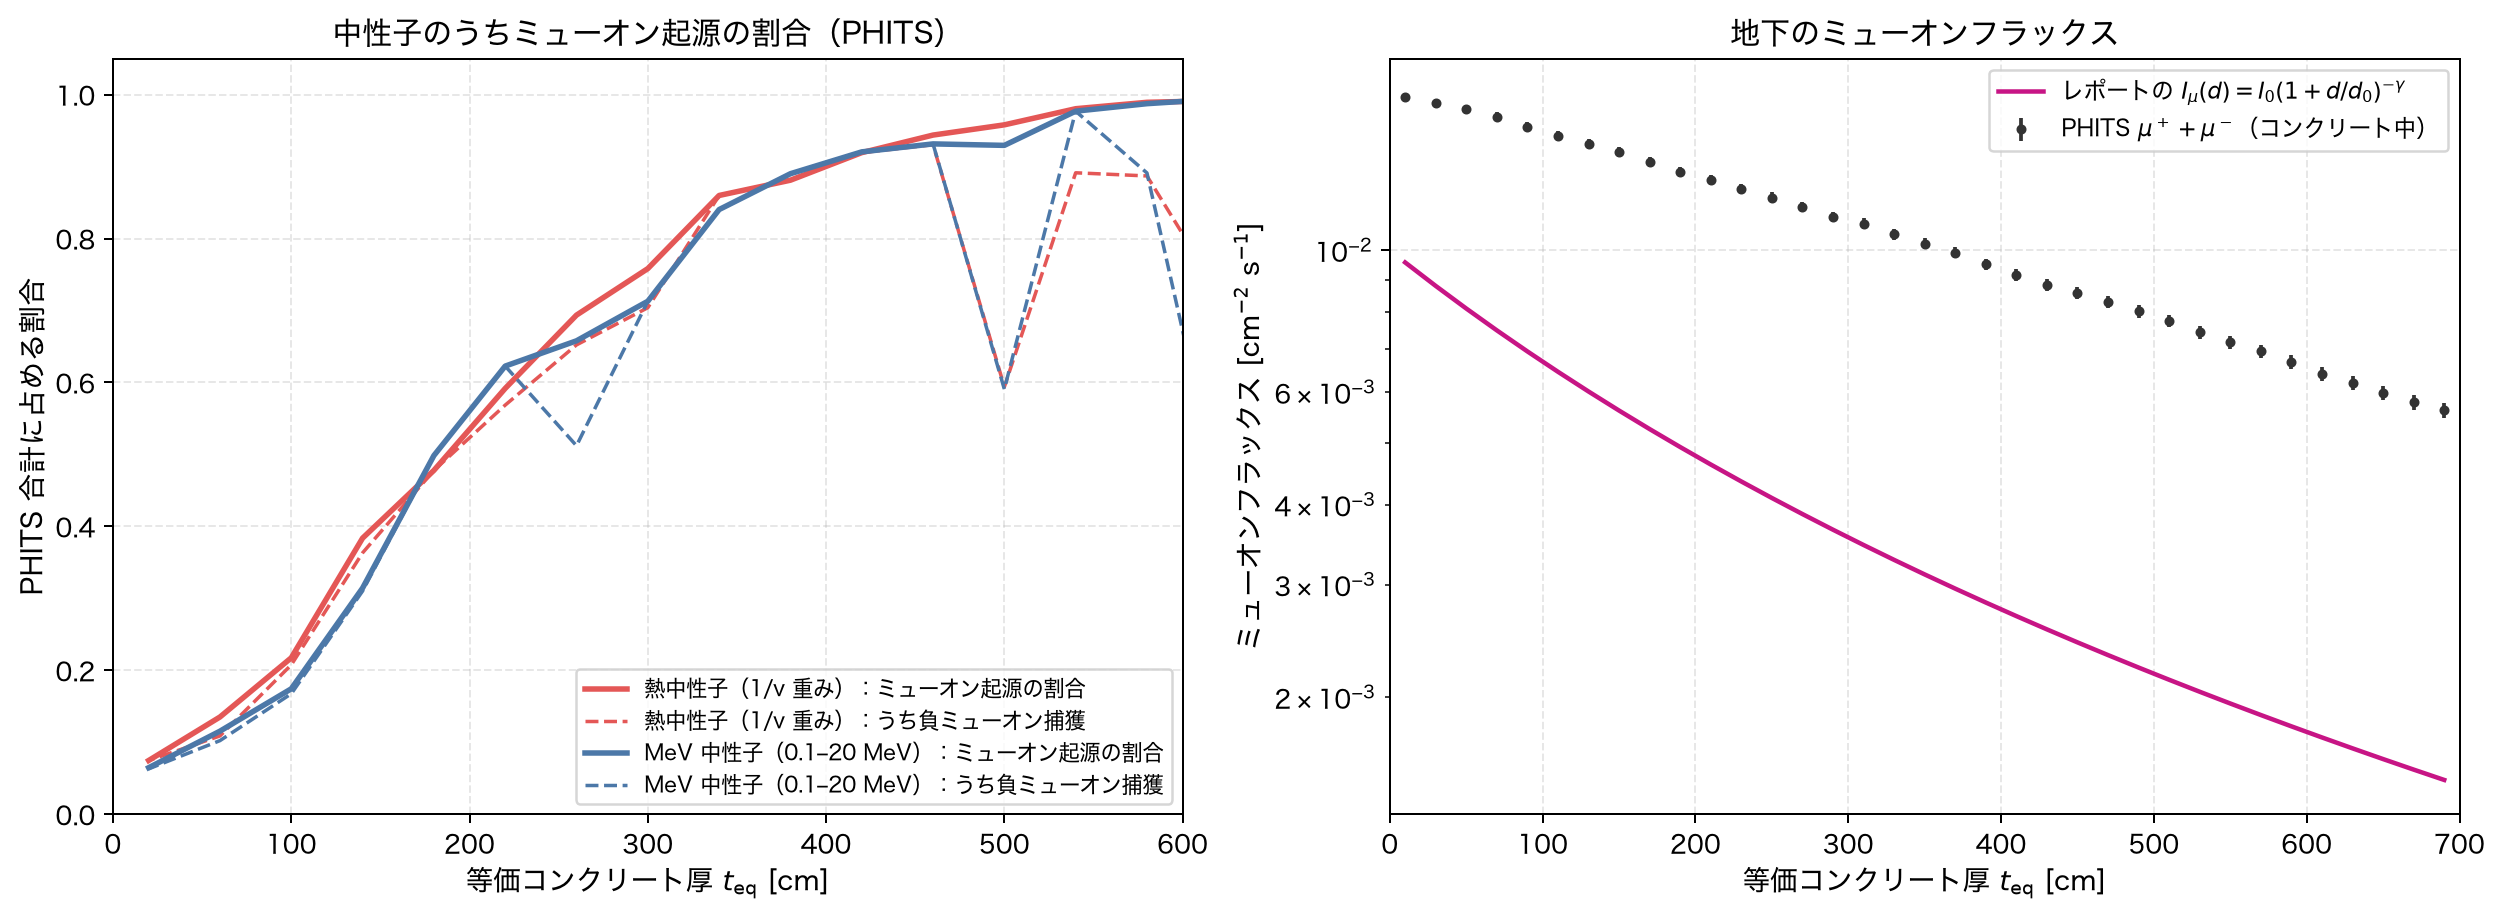
\includegraphics[width=\linewidth]{figures/fig12_phits_fraction_muflux.png}
  \caption{左：PHITS の中性子フラックスに占めるミューオン起源（実線）と負ミューオン捕獲（破線）の割合。
  右：PHITS で求めたコンクリート中のミューオンフラックスと，\ref{sec:model}節の $I_\mu(d)$ の比較。}
  \label{fig:phitsfrac}
\end{figure}

\subsection{検出器の応答と地点の体系を含めた PHITS による予測}
\label{sec:phitsmodel}

前節の比較には3つの近似が入っていた。
(a) 検出器の応答を $1/v$ の重みや 0.1--20\,MeV の窓で代用したこと，
(b) 地点の遮蔽を一様なコンクリートの半無限体系で表し，検出器を物質の中に置いたこと，
(c) 実測を，メーカー感度と転送較正による $\eSpk$ で割ったフラックスとして比べたこと，である。
ここでは PHITS で4台の管の応答関数を求め，地点ごとの遮蔽の積層と部屋（空洞）を含む体系で計算した中性子スペクトルと畳み込んで，
各管の peak ROI の計数率を直接予測した。この比較には $\eSpk$ も転送較正も使わない。

\paragraph{検出器の応答関数}
4台の管を，SUS 製の管壁（厚さ 0.2\,cm），有感部の \He（10\,atm）と両端の不感部に分けて模擬した。
PE 付き管は，D2 が外径 29\,cm・高さ 80\,cm の PE 容器（中の穴は半径 7.5\,cm，穴の中は空気），
d2 が管に密着した外径 15.5\,cm・長さ 49.5\,cm の PE で，どちらも上下を PE で閉じている（中の管はそれぞれ D1，d1 と同じ型）。
管を中心とする球面から等方的に単色の中性子を入射し（$5\times10^{-9}$--$10^{3}$\,MeV の19点），
有感部での飛跡長に \He(n,p) の断面積（0.0253\,eV で 5333\,b の $1/v$）と原子数密度を掛けて反応率を求め，
入射フルエンスで割った値を応答 $R_{\mathrm{det}}(E)$ [cm$^2$] とした（図\ref{fig:resp}）。
予測計数率は $f_{\mathrm{peak}}\sum_E R_{\mathrm{det}}(E)\,\phi(E)$ で，中性子スペクトル $\phi(E)$ にはエネルギーについて対数補間した応答を掛けた。

熱中性子（0.0253\,eV）に対する等方入射の応答は D1 で 324\,cm$^2$，d1 で 98.5\,cm$^2$ であり，
メーカー感度（450，123\,cps/nv）の 0.72 倍と 0.80 倍であった。
メーカー値は一方向からの入射で決めた値と考えられ，等方的な場では有効な面積が小さくなる。
d1 の値は，黒鉛パイルでの直接測定（85.2，81.7\,cm$^2$，\ref{sec:sys}節）に近い。
また \He の熱中性子に対する吸収は強く（有感部の径の中でほぼ吸収される），熱領域の応答は管の断面積で頭打ちになるため，
裸管の応答は 1--100\,eV では $1/v$ の外挿より数倍大きい。
PE 付き管の応答は D2 で 2\,MeV 付近に最大（168\,cm$^2$），d2 で 1\,MeV 付近に最大（46\,cm$^2$）をもち，
熱中性子に対する応答は D2 で 8.7\,cm$^2$，d2 で 4.8\,cm$^2$ と裸管の 1/40--1/20 である。

\begin{figure}[htbp]
  \centering
  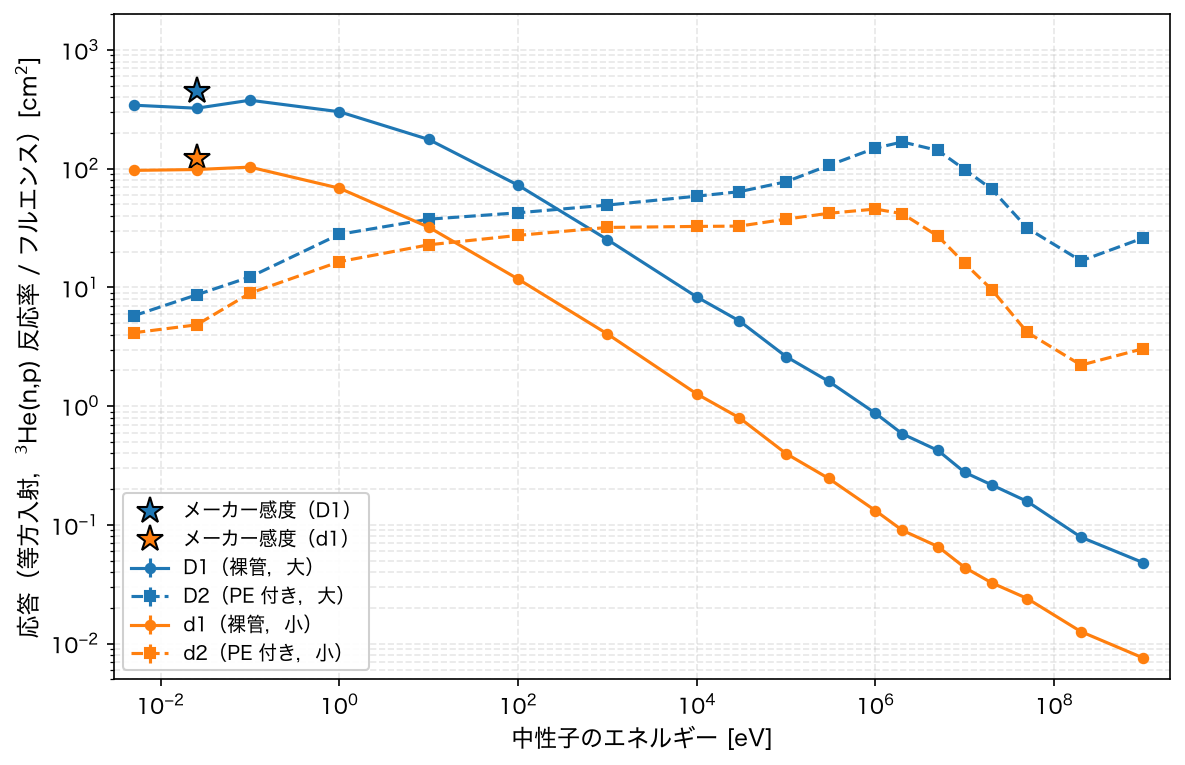
\includegraphics[width=0.72\linewidth]{figures/fig13_response.png}
  \caption{PHITS で求めた4台の管の応答関数（等方入射，\He(n,p) の反応率をフルエンスで割った値）。
  実線は裸管，破線は PE 付き管，星印はメーカー感度。誤差棒は統計誤差（ほとんどが記号より小さい）。}
  \label{fig:resp}
\end{figure}

管の中と周りで中性子がどう振る舞うかを，管の軸を通る断面のフラックス分布で図\ref{fig:detmap}に示す。
上段は 1\,MeV の中性子を等方的に入射したときの熱中性子成分である。
PE の中では減速された熱中性子が溜まって入射フルエンスの 0.6--0.7 倍に達するが，管の有感部の中では D2 で約 0.02 倍，d2 で約 0.06 倍まで下がる。
PE で熱化した中性子が，管壁のすぐ内側で \He に吸収されていることがわかる。
下段は熱中性子を入射した裸管で，管の外ではフラックスが入射フルエンスとほぼ等しい（0.93 倍）のに対し，管の中心では D1 で約 $6\times10^{-4}$ 倍，d1 で約 0.015 倍まで減る。
10\,atm の \He 中での熱中性子の平均自由行程は約 0.75\,cm なので，熱中性子は有感部の表面から 1\,cm 程度でほとんど吸収される。
上で述べた「熱領域の応答が管の断面積で頭打ちになる」ことは，この様子に対応している。

\begin{figure}[htbp]
  \centering
  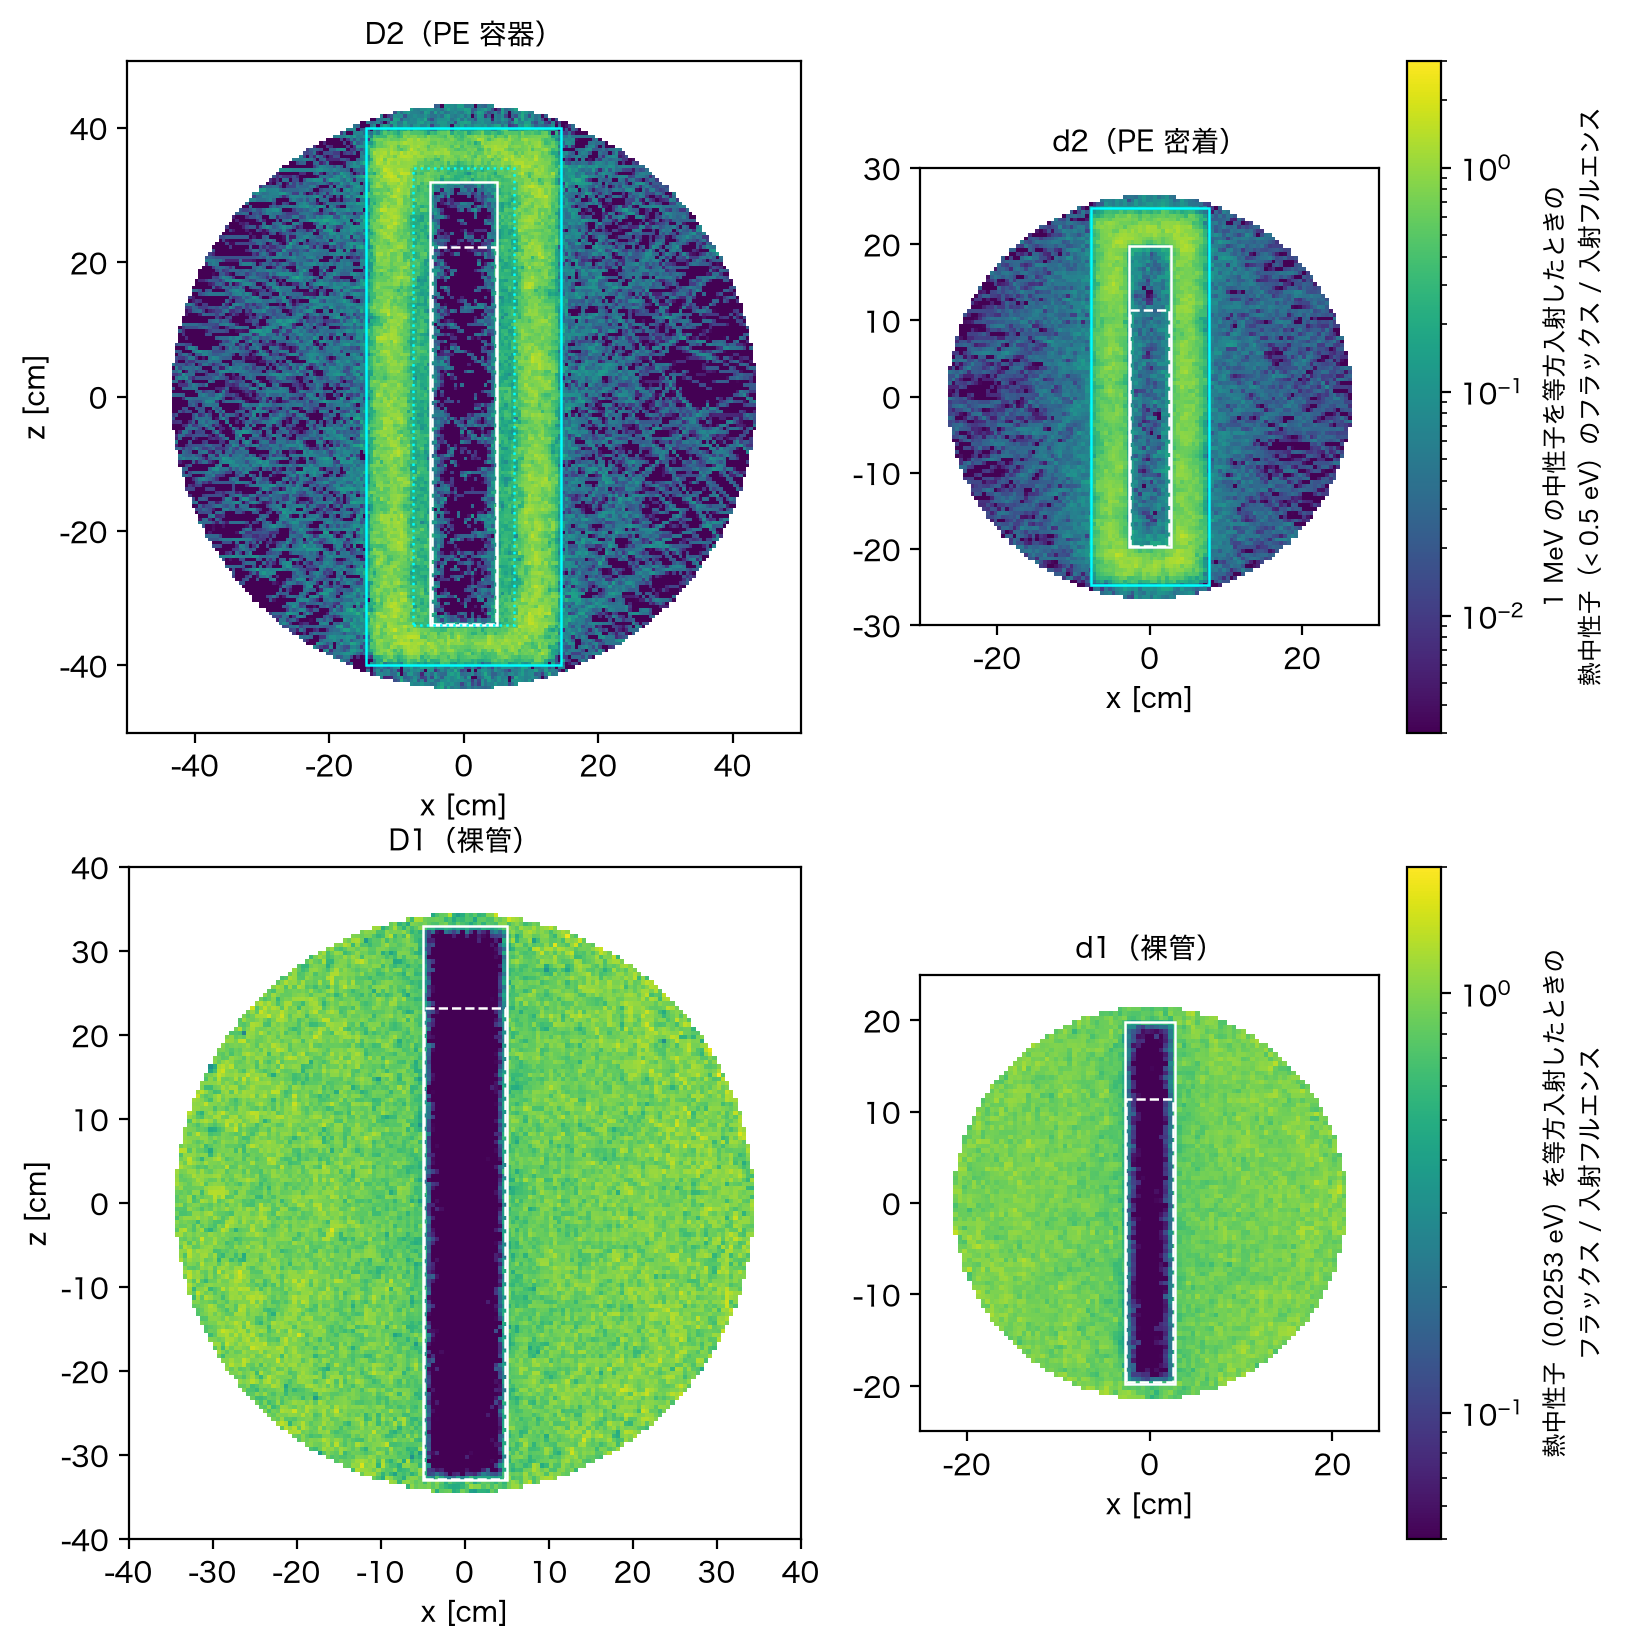
\includegraphics[width=0.82\linewidth]{figures/fig15_phits_detectors.png}
  \caption{PHITS で計算した，管の軸を通る断面（厚さ 1\,cm）での中性子フラックスの分布（入射フルエンスとの比）。
  上段：PE 付き管に 1\,MeV の中性子を等方入射したときの熱中性子（$<0.5$\,eV）成分。下段：裸管に熱中性子（0.0253\,eV）を等方入射したとき。
  白の実線は SUS 管，白の破線は有感部（その上は不感部），水色の実線は PE，水色の点線は D2 の PE 容器の穴。円の外は線源球の外で計算していない。}
  \label{fig:detmap}
\end{figure}

\paragraph{地点ごとの体系}
地表から下に，表\ref{tab:sites}の垂直方向の積層（コンクリートと土）を置き，その直下に幅 3\,m・高さ 3\,m・長さ 20\,m の空気の部屋を置いた。
部屋の壁と床の下はコンクリートである。部屋全体の空気中で平均した中性子スペクトルを応答関数と畳み込んだ。
土は乾燥した鉱物と水の混合とし，水の質量分率を関東ローム 0.50（密度 1.35\,g\,cm$^{-3}$），常総層 0.27（1.65），下総層群 0.19（1.85）とした。
比較のため，土を本文の組成（水素 2\,wt\%）とした計算も行った。
テストホール，PF，放射線棟 BT，PS，KEKB はこの体系で，Linac3 は\ref{sec:phitscomp}節の天井厚 300\,cm のトンネルの計算を用いた
（$\mu^+$ の成分は計算していないので，同じ深さのコンクリート中の $\mu^+/\mu^-$ 比で補った）。
K2K は，半無限コンクリート中の値に PS の部屋/コンクリート中の比を成分ごとに掛けて求めた。
計算量は，1地点あたり $\mu^-$ が約 $1\times10^{4}$--$2\times10^{4}$ 個，$\mu^+$ が約 $4\times10^{3}$--$5\times10^{3}$ 個，ハドロンが約 $6\times10^{3}$--$1.2\times10^{4}$ 個である。

この体系の中で中性子がどう分布するかを見るため，浅い PF と深い PS について，同じ体系に断面のメッシュタリーを加えて統計を増やした計算
（1地点あたり $\mu^-$ $6\times10^{4}$ 個，ハドロン $4\times10^{4}$ 個）を行った（図\ref{fig:sitemap}）。
大気由来のハドロンによる中性子（左列）は，地表から下へ急に減り，PS の部屋の中では地上の空気中の約 1/360（$1.4\times10^{-5}\,\flux$）になる。
PF では部屋の中（$1.4\times10^{-3}$）の方が同じ高さの横のコンクリート中（$4.2\times10^{-4}$）より大きい。
部屋の上には天井 105\,cm しかないが，横の同じ高さの点の上には 1--4\,m のコンクリートがあるためで，天井を抜けた中性子が空気の部屋の中を減衰せずに広がる様子が見える。
一方，負ミューオンによる中性子（右列）は深さによらずほぼ一様で（$2$--$5\times10^{-4}\,\flux$），PS の部屋の中ではハドロンによる中性子の約 24 倍になる。
深い地点の中性子の大部分がミューオン起源であること（\ref{sec:phitscomp}節）が，断面の分布としても確かめられる。
また PS の部屋の中の負ミューオン起源の中性子（$3.3\times10^{-4}$）は横のコンクリート中（$2.2\times10^{-4}$）の約 1.5 倍で，
深い地点では空洞がフラックスを上げる向きにはたらくこと（後述）とも対応している。

\begin{figure}[htbp]
  \centering
  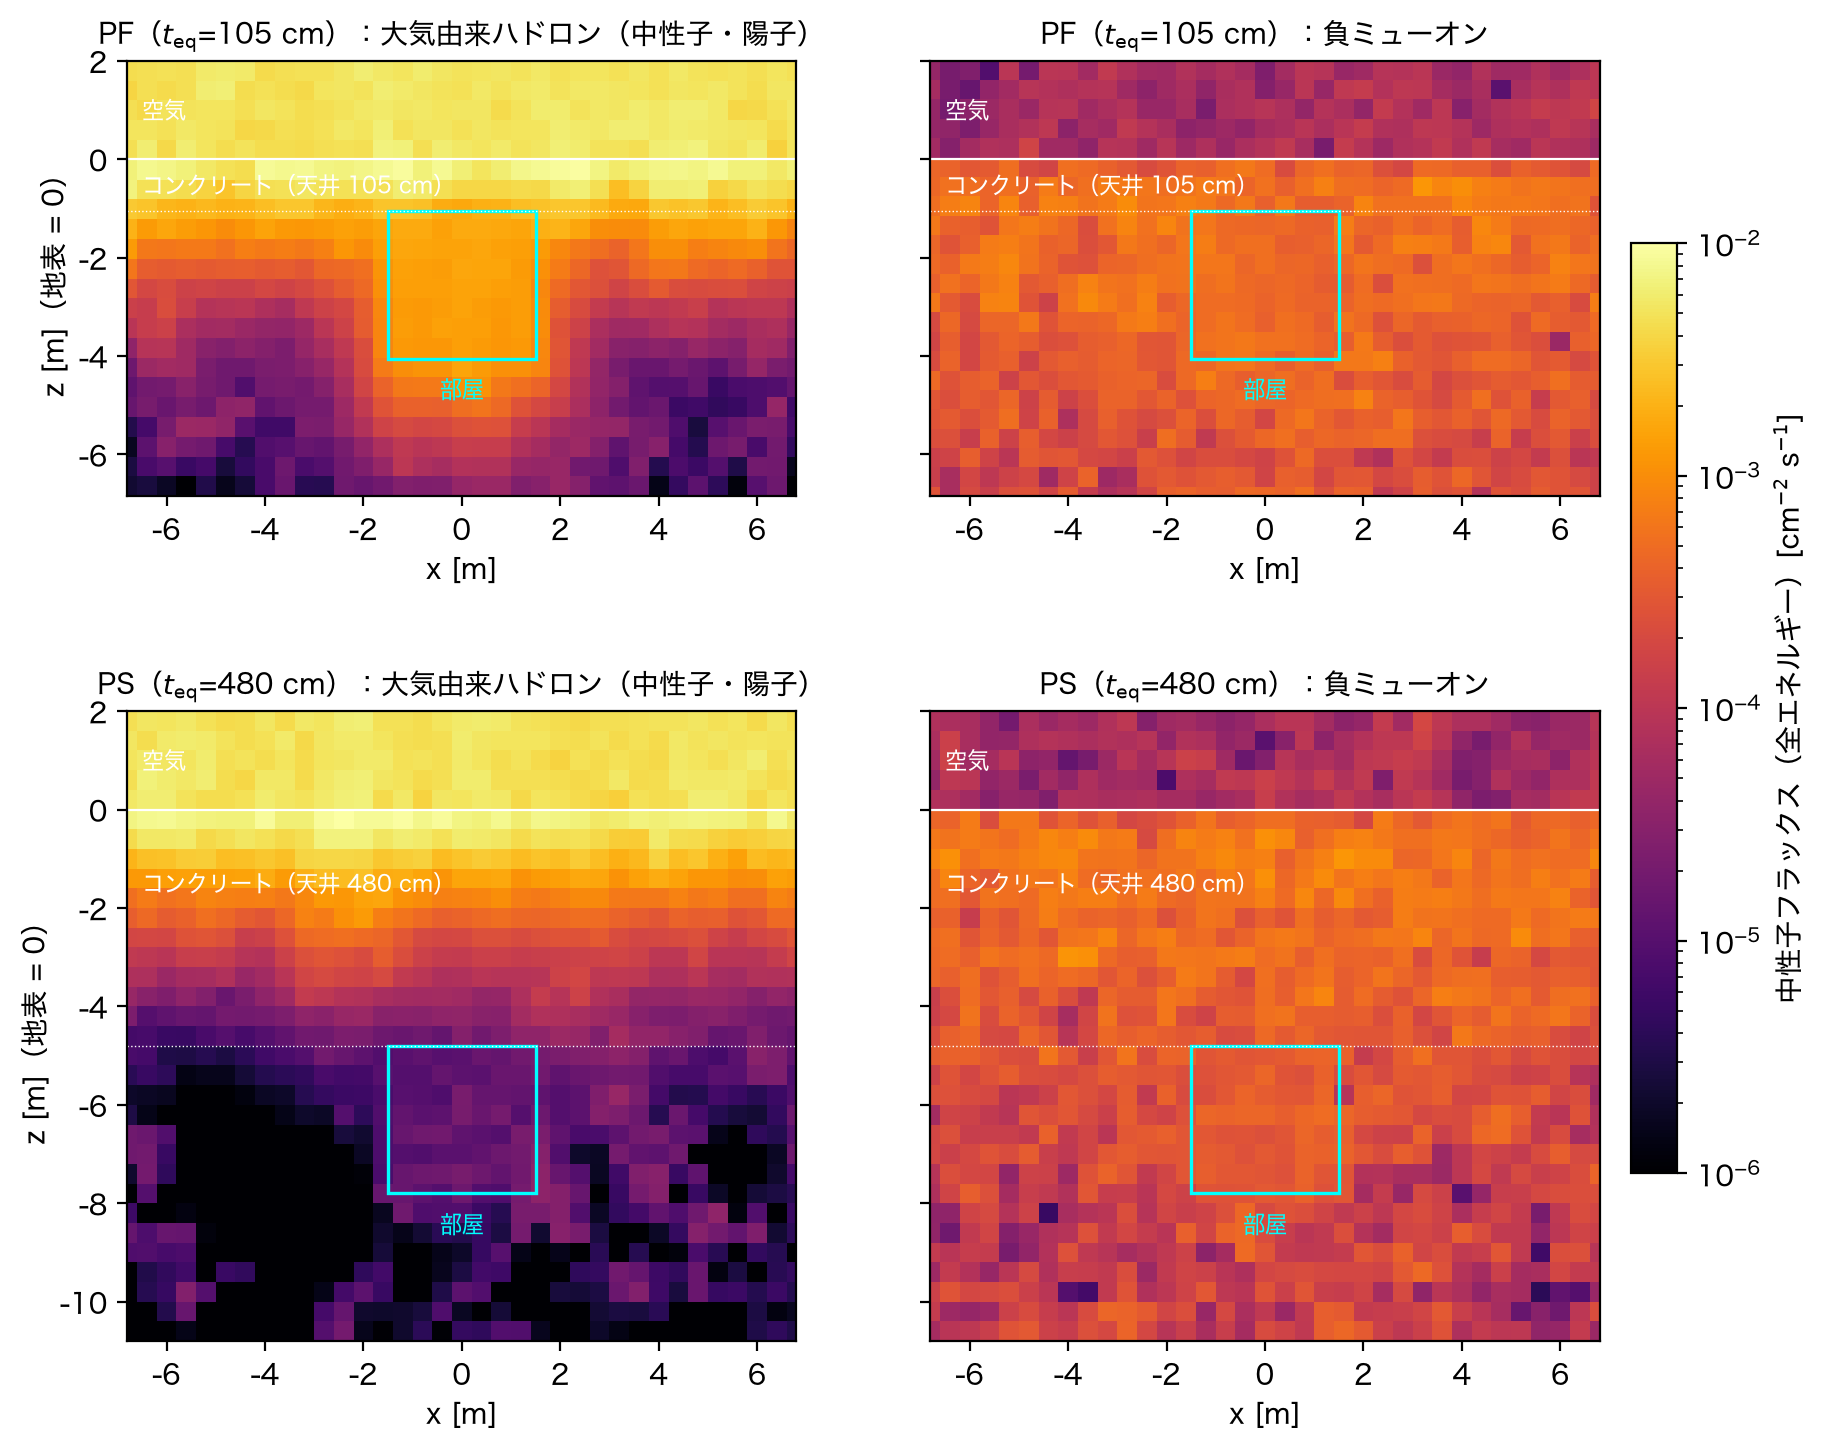
\includegraphics[width=0.9\linewidth]{figures/fig14_phits_sites.png}
  \caption{PHITS で計算した地点体系の断面（部屋の長さ方向に平均）での中性子フラックス（全エネルギー）。
  上段：PF（コンクリート 105\,cm），下段：PS（コンクリート 480\,cm）。左列：大気由来のハドロン（中性子・陽子）を線源としたとき，右列：負ミューオンを線源としたとき。
  白の実線は地表，白の点線は天井（部屋の上面の高さ），水色の枠は部屋。左下の深部の黒い斑は統計が足りない領域である。
  左列は 20\,cm のメッシュを 40\,cm にまとめて表示した。}
  \label{fig:sitemap}
\end{figure}

\paragraph{自由パラメータなしの比較}
結果を図\ref{fig:phitsmodel}左に，各点の数値を付録の表\ref{tab:phitsmodel}に示す。
部屋の中の予測は，同じ深さのコンクリートの中の値に比べ，浅い地点（テストホール，PF，BT）で 0.5--0.8 倍と小さかった。
大気由来の中性子が主な深さでは，空洞の中にはまわりの物質で減速された中性子の一部しか届かないためである。
一方，ミューオン起源が主な深い地点（PS，KEKB）では 0.7--1.7 倍で，PE 付き管ほど大きくなった。
深部では中性子がまわりのコンクリート全体でほぼ一様に作られるので，空洞の中には四方の壁からの中性子が減速・吸収されずに集まり，
とくに減速される前の MeV 中性子が物質中より多くなるためと考えられる。
このように空洞の効果は，浅い地点ではフラックスを下げ，深い地点では上げる向きにはたらく。
ただしその大きさは 2 倍未満で，深部に残る実測との差を空洞の効果だけで説明することはできない。

$\eSpk$ を使わずに計数率そのものを比べると，
PF・BT・PS の裸管，Linac3 の d1，BT の d2 の6点は実測/PHITS $=0.82$--1.33 で，自由パラメータなしで 1.4 倍以内に合った。
とくに PF（0.87），BT（1.07），PS（0.98）の D1 は 15\% 以内で一致しており，
PHITS の応答関数と地点の体系が，浅い地点から深い地点まで裸管の絶対計数率を較正なしに再現できる場合があることを示している。
ただし予測には d1 のピーク窓の割合 $f_{\mathrm{peak}}$ を D1 にも用いており，D1 の実際の割合が大きければ D1 の実測/PHITS は 0.7--0.8 程度まで下がりうる（\ref{sec:sys}節）。
一方，テストホールの裸管は 0.43--0.44 と PHITS の方が約2倍大きい。
テストホールは $\teq=57$\,cm と浅く大気由来の成分が主なので，天井の積層や部屋の大きさ・開口の模型化に敏感であることが考えられる。
また，KEKB（D1 1.98，d2 2.00），K2K（D2 1.96），PF の D2（2.27），Linac3 の D1（1.84）では実測が PHITS を約2倍上回り，
Linac3 の PE 付き管（D2 7.8，d2 3.7）ではさらに大きく上回った。
PE 付き管と裸管の計数率の比（D2/D1）は，実測が地上・PF・Linac3 で 0.56--0.70 とほとんど変わらないのに対し，
PHITS では部屋の中で 0.22--0.35，Linac3 のトンネルで 0.16 である。


\paragraph{PHITS に基づくモデル}
この予測を土台に，各点の計数率を
\begin{equation}
  R_{\mathrm{pred}} = k_{\mathrm{type}}\,\bigl(H + r\,M\bigr)
  \label{eq:phitsmodel}
\end{equation}
と表すモデルを当てはめた。$H$ と $M$ は PHITS による大気由来ハドロンとミューオン起源（負ミューオン捕獲＋高速ミューオン）の予測計数率，
$k_{\mathrm{type}}$ は裸管と PE 付き管ごとの規格化（応答の模型化と較正の誤差を吸収する），$r$ はミューオン起源の倍率である（PHITS そのままなら $r=1$）。
当てはめは対数の残差で行い，各点の誤差は実測の統計誤差・PHITS の統計誤差・モデルの系統誤差 10\% の二乗和とした。
比較のため，$r=1$ に固定して管の大きさ（大径 D1/D2，小径 d1/d2）ごとに一定の計数率 $B$ を加えたモデル
$R_{\mathrm{pred}}=k_{\mathrm{type}}(H+M)+B_{\mathrm{size}}$ も当てはめた。
結果を図\ref{fig:phitsmodel}右に，当てはめの数値を付録の表\ref{tab:phitsfit}に示す。


\begin{figure}[htbp]
  \centering
  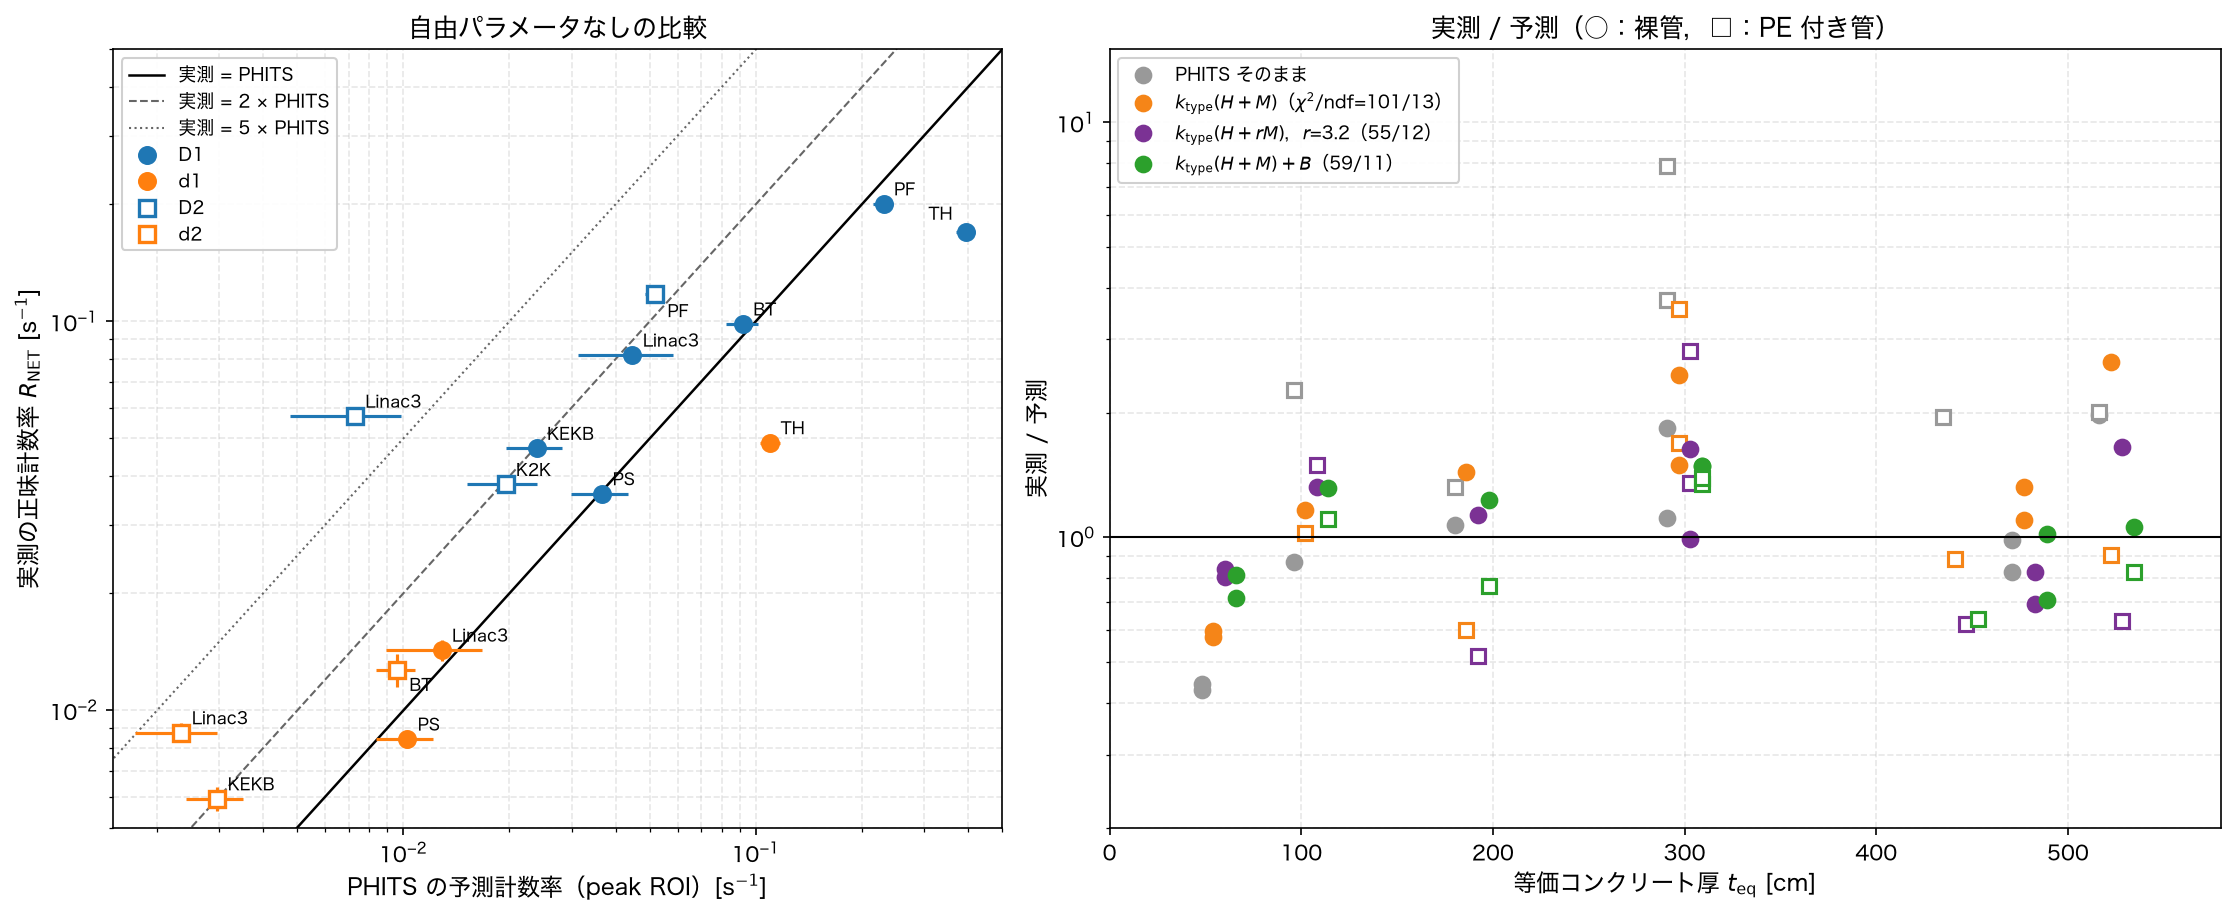
\includegraphics[width=\linewidth]{figures/fig13_phits_model.png}
  \caption{左：peak ROI の計数率の実測と，PHITS の予測（応答関数×地点の体系，自由パラメータなし）の比較。
  ○は裸管，□は PE 付き管，青は大径管，橙は小径管。実線は一致，破線と点線は実測が 2 倍，5 倍の線。
  右：実測/予測を等価コンクリート厚に対して示したもの。灰：PHITS そのまま，橙：$k_{\mathrm{type}}(H+M)$，
  紫：$k_{\mathrm{type}}(H+rM)$，緑：$k_{\mathrm{type}}(H+M)+B$（見やすさのため横に少しずらした）。}
  \label{fig:phitsmodel}
\end{figure}

$r=1$ のまま規格化だけを合わせると，$k_{\mathrm{bare}}=0.75$，$k_{\mathrm{PE}}=2.2$ となり，$\chi^2/\mathrm{ndf}=101/13$ と深い地点の差が残る。
$k_{\mathrm{bare}}$ が1より小さいのは，PHITS が実測の約2倍となったテストホールの2点に引かれるためで，
PF・BT・PS の裸管だけを見れば PHITS の絶対値そのままでよい。
$r$ を自由にすると $r=3.2\pm0.7$ で $\chi^2$ はほぼ半分になり，15点の実測/モデルは 0.52--2.8（Linac3 の D2 を除くと 0.52--1.65）に収まる。
土の組成と Linac3 の天井の厚さを変えても $r=3.0$--4.0 で，結論は変わらない。
ただし，$r\approx3$ はミューオン起源の中性子が PHITS の3倍あることを意味する。
PHITS の負ミューオン捕獲あたりの中性子の数（約 1.2 個，\ref{sec:phitscomp}節）と地下のミューオンフラックスの両方がそれほど大きく外れているとは考えにくく，
$r$ は物理量というより，深い地点に残る差をまとめて吸収した量とみるべきである。

一定成分のモデルも $\chi^2$ を 59/11 まで下げるが，$B_{\mathrm{large}}/B_{\mathrm{small}}\approx11$ で，大径管と小径管の有感部の体積の比（約 6.5）とは一致しない。
Linac3 で実測から PHITS を引いた残りも，D1 0.037，D2 0.050，d1 0.0015，d2 0.0065\,s$^{-1}$ と管ごとにばらばらで，
「管の型ごとに一定の，中性子によらない計数」を示す証拠にはならない。
実測が PHITS を約2倍以上上回る点のうち，Linac3 と KEKB は低チャンネルのノイズのために部分補正（$1/f$ 倍，1.41--1.50 倍）を適用したスペクトルであるが，
補正を適用していない PF の D2 も PHITS を約2倍上回り（参考値の K2K も同様），逆に補正を適用した PS の裸管は PHITS と一致している。
したがって，部分補正だけで残りの差を説明することはできない。

\paragraph{KEKB と PS}
KEKB（$\teq=525$\,cm）は PS（480\,cm）より深いにもかかわらず，D1 の計数率は KEKB の方が 1.31 倍大きい。
PHITS は逆に KEKB を PS の 0.65 倍と予測しており，実測/PHITS は PS 0.98 に対し KEKB 1.98 と2倍違う。
KEKB の遮蔽は大部分が土（670\,cm）で $\teq$ の不確かさも最大（$\delta\teq=81$\,cm）なので，土の厚さや含水量の見積もり，あるいはトンネル近くの立坑などの垂直積層で表せない経路が，KEKB で $\teq$ を過大に見積もっている可能性がある。
地点の遮蔽を一次資料で確かめることが，この差を解く最初の手がかりになる。

\paragraph{手調整の多成分モデルとの関係}
\ref{sec:model}節の多成分モデルが深部で与えるミューオン起源の成分 $f_1$ は，PHITS の半無限コンクリート中のミューオン起源の MeV 中性子フラックスの
約2--3倍（BT 1.8，PF 3.1，Linac3 2.4，KEKB 3.0 倍）である。
多成分モデルは PE 付き管の転送較正済みのフラックスに手で合わせたもの，ここでの $r$ は計数率を較正なしに当てはめたものと，出発点は異なるが，
どちらも「PHITS のミューオン起源成分をおよそ3倍にすると実測の深さ依存に合う」という同じ結論になった。
多成分モデルの大きな収量 $Y_n$（Wang らの式の約20倍，\ref{sec:phitscomp}節）は，この倍率を含んでいると解釈できる。
一方，多成分モデルの一定成分 $f_3=3.9\times10^{-6}\,\flux$ に対し，一定成分モデルの $B$ をフラックスに換算すると
（$B/\eSpk$），大径管で $1.2$--$1.8\times10^{-4}$，小径管で $0.4$--$0.9\times10^{-4}\,\flux$ と $f_3$ の 10--50 倍になり，深部のフラックスそのものと同程度である。
したがって $B$ は大地由来の $(\alpha,n)$・自発核分裂のような一定成分ではなく，深部の差をまとめて吸収した量であり，
その点で $r$ を自由にしたモデルと同じ情報しか含んでいない。

どちらのモデルも $\chi^2/\mathrm{ndf}=4$--6 で，10\% の系統誤差を仮定しても統計的には合っていない。
PHITS で説明できるのは PF・BT・PS の裸管の絶対値と，深部の計数率がミューオン起源でほぼ決まることまでであり，
深部に残る約2倍の差（Linac3 の PE 付き管ではさらに大きい）とテストホールの逆向きの差は，地点ごとの幾何
（Linac のクライストロンギャラリーへの貫通孔やシャフトなど，垂直積層で表せない経路）と PE 付き管の応答の模型化の両面から調べる必要がある。

\subsection{系統誤差と本研究の限界}
\label{sec:sys}

\paragraph{実効面積の絶対値}
裸管の $\varepsilon S_{\mathrm{total}}$ にはメーカー感度を用いた。
黒鉛パイルでの d1 の直接測定では $R/\phi=85.2$\,cm$^2$（30\,cm），81.7\,cm$^2$（80\,cm）となり，メーカー値 123\,cm$^2$ より約 32\% 小さい。
パイルの値を使うとすべての絶対フラックスが約 1.47 倍になる。パイル測定の不感時間（4--9\%）や，黒鉛パイルが文献当時と同じ状態かどうかも確認できていない。
PHITS で求めた等方入射の熱中性子応答（D1 324\,cm$^2$，d1 98.5\,cm$^2$，\ref{sec:phitsmodel}節）はメーカー値の 0.72 倍と 0.80 倍で，
等方的な場ではメーカー値で割ったフラックスが 1.25--1.4 倍程度小さく出ている可能性がある。
PHITS の等方応答を実効面積に用いた場合の熱中性子フラックスを表\ref{tab:fluxphits}に併記する
（D1 は $450/324=1.39$ 倍，d1 は $123/98.5=1.25$ 倍になる。PE 付き管は D1 から転送しているので D1 と同じく 1.39 倍になる）。
地上の D1 は $2.35\times10^{-3}\,\flux$ となり，昨年度の屋外の値より約 40\% 大きくなる。
なお昨年度の値は黒鉛パイルでの実測（$\varepsilon S\approx88$--92\,cm$^2$）で較正されているので，今年度もパイルを基準にすると（上記の 1.47 倍）地上の D1 は約 $2.5\times10^{-3}\,\flux$ となり，やはり昨年度より約 45\% 大きい。
昨年度との比較は，どの実効面積を用いるかで 1\% から 45\% まで変わることになる。
また倍率が管ごとに違うので，同じ地点の D1/d1 比は 1.11 倍になり（テストホール 1.06，管理棟2階 1.28，PS 1.30，Linac3 1.74），
大径管と小径管の一致はメーカー値のときよりやや悪くなる。
どちらの実効面積が正しいかは，等方的な熱中性子場（黒鉛パイルの中など）での同時測定で決める必要がある。
ただし，地上比で表した相対フラックスはこの影響を受けない。

\begin{table}[htbp]
  \centering
  \caption{熱中性子フラックスの実効面積による違い [$\flux$]。「メーカー」は本文の値，「PHITS」は PHITS の等方応答を用いた値。}
  \label{tab:fluxphits}
  \small
  \begin{tabular}{lrrrrr}
    \toprule
    & & \multicolumn{2}{c}{D1} & \multicolumn{2}{c}{d1} \\
    \cmidrule(lr){3-4}\cmidrule(lr){5-6}
    地点 & $\teq$ [cm] & メーカー & PHITS & メーカー & PHITS \\
    \midrule
    地上 & 0 & $1.69\times10^{-3}$ & $2.35\times10^{-3}$ & --- & --- \\
    管理棟2階 & --- & $2.08\times10^{-3}$ & $2.89\times10^{-3}$ & $1.81\times10^{-3}$ & $2.27\times10^{-3}$ \\
    管理棟1階 & --- & $1.49\times10^{-3}$ & $2.08\times10^{-3}$ & --- & --- \\
    テストホール & 57 & $6.61\times10^{-4}$ & $9.18\times10^{-4}$ & $6.97\times10^{-4}$ & $8.70\times10^{-4}$ \\
    PF & 105 & $7.83\times10^{-4}$ & $1.09\times10^{-3}$ & --- & --- \\
    放射線棟 BT & 189 & $3.85\times10^{-4}$ & $5.34\times10^{-4}$ & --- & --- \\
    Linac3 & 300 & $3.20\times10^{-4}$ & $4.44\times10^{-4}$ & $2.04\times10^{-4}$ & $2.55\times10^{-4}$ \\
    PS & 480 & $1.41\times10^{-4}$ & $1.96\times10^{-4}$ & $1.21\times10^{-4}$ & $1.51\times10^{-4}$ \\
    KEKB & 525 & $1.84\times10^{-4}$ & $2.56\times10^{-4}$ & --- & --- \\
    \bottomrule
  \end{tabular}
\end{table}

\paragraph{D1 のピーク窓の割合}
D1 の $\eSpk$ には，d1 のパイル測定から求めたピーク窓の割合（0.5695）を用いた（\ref{sec:calib}節）。
しかし同じ管理棟2階で測った壁効果窓とピーク窓の計数の比は，D1 で 1.22，d1 で 1.59 と大きく異なる。
径の大きい D1 では壁効果が相対的に小さく，全計数に占めるピーク窓の割合が d1 より大きいためと考えられる。
壁効果窓の計数が全計数に占める割合が両管で同程度とすると，D1 のピーク窓の割合は d1 の約 1.3 倍となり，
D1 の絶対フラックスは約 1.3 倍過大（真の値は本文の値の約 0.77 倍），PHITS による D1 の予測計数率は約 1.3 倍過小になる（D1 の実測/PHITS は PF・BT・PS で 0.7--0.8 程度）。
実際，地上の D1 を壁効果窓で求めると $1.32\times10^{-3}\,\flux$ で，ピーク窓の値より約 22\% 小さい。
D1 のパイル 80\,cm の測定などから D1 自身の窓の割合を決めることが必要である。
地上比などの同じ検出器どうしの比は，この影響を受けない。

\paragraph{PE 付き管の転送較正}
d2 の $\eSpk$ は，転送に使う窓や地点の選び方によって 27--55\,cm$^2$ の幅がある。
また Linac で D1 にそろえた D2 は，地上では D1 の 0.81 倍となり（\ref{sec:det}節），PE 付き管と裸管の応答比は地点によって 20\% 程度変わる。
このため MeV 中性子の絶対値は熱中性子より不確かである。
さらに，この較正は転送地点で PE 付き管と裸管のフラックスが等しいと置くことに相当するので（\ref{sec:calib}節），
PE 付き管の値は MeV 中性子の真の絶対フラックスではない。MeV 中性子の絶対値を得るには，既知のエネルギー分布の場での直接較正が必要である。

\paragraph{深部で PHITS を上回ること}
PHITS の成分別の計算（\ref{sec:phitscomp}節）では，深部の MeV 中性子の実測が計算を 1.7--3.0 倍上回り，
トンネルの空洞を入れても差は縮まらなかった（熱中性子は 1.0--1.4 倍でほぼ一致）。
応答関数と地点の体系を含めて計数率を直接比べると（\ref{sec:phitsmodel}節），$\eSpk$ と転送較正の不確かさは取り除かれ，
PF・BT・PS の裸管は 15\% 以内で合ったが，KEKB・Linac3・K2K と PF の D2 では約2倍以上の差が残り，テストホールでは逆に PHITS が約2倍大きかった。
残る差の候補は，垂直積層で表せない幾何（貫通孔・シャフト・側方の薄い遮蔽），土の厚さと含水量（とくに KEKB），PE 付き管の応答の模型化である。
部分補正を適用したスペクトルとそうでないスペクトルの両方で差が見られるので，部分補正だけが原因とは考えにくい。
加速器のビームに由来する中性子は，測定期間中に加速器が運転していなかったので原因から除外できる（\ref{sec:source}節）。

\paragraph{遮蔽厚の見積もり}
$\teq$ は図面から読み取った垂直方向の厚さである。例えば Linac の遮蔽は，教材では 250\,cm，本解析では 300\,cm としており，一次資料での確認が必要である。
斜めに入射する宇宙線は垂直厚より長い経路を通る。天頂角分布が $\cos^2\theta$\cite{Gaisser2016}のとき，
水平面を横切る粒子で平均した経路長は垂直厚の約 1.3 倍（$\langle1/\cos\theta\rangle=4/3$）になる。
単純指数減衰の予測と多成分モデルではこの効果を考慮していないが，PHITS の計算は線源の角度分布を含むので，PHITS との比較にはこの効果が入っている。

\paragraph{部分補正とデータの質}
深部のスペクトルに適用した $1/f$ 補正（1.41--1.50 倍）は，パイルでのスペクトルの形が深部でも同じであることを仮定している。
この補正が二重にかかる誤りは修正したが（\ref{sec:partial}節），補正の仮定そのものの不確かさは残る。
また，D2 のテストホールは D1 との重複データ，K2K（D2）はノイズが強い。d1 のテストホールには，ライブタイムが同じで計数の異なるファイルが2つあり，一方だけを用いた。

\paragraph{モデルの係数}
多成分モデルの係数は手で調整したもので，組成の係数の組と $\beta$ も熱中性子用（5成分，$\beta=0.84$）と MeV 中性子用（6成分，$\beta=0.90$）で異なる。
係数の不確かさを評価していないので，RMS 0.048\,dex はモデルの予測精度を表すものではない。
係数を物理的に決めるには，$I_\mu$ の実測や PHITS の成分別計算（\ref{sec:phitscomp}節）を用いる必要がある。

\paragraph{PHITS の体系と応答}
\ref{sec:phitscomp}節の成分別計算は一様なコンクリートの半無限体系で行ったが，
\ref{sec:phitsmodel}節では地点ごとの積層（土の含水量を含む）と部屋を入れ，検出器の応答関数と直接畳み込んだ。
土を含水組成から本文の組成に変えても当てはめの結論は変わらなかった（付録の表\ref{tab:phitsfit}）。
残る近似は，(i) 部屋を幅 3\,m・高さ 3\,m の直方体とし，実際の断面・側方の遮蔽・貫通孔を入れていないこと，
(ii) 検出器を部屋全体の空気中の平均スペクトルで代表させたこと，(iii) 応答関数で PE 容器や管の構造を簡略化し，
peak ROI の割合 $f_{\mathrm{peak}}$ をすべてのエネルギーで同じとし，D1 にも d1 の値を用いたこと，(iv) 深い地点の予測の統計誤差が 18--35\% あること，である。
地上は地面と建物の模型が粗く，比較から除いた。

%======================================================================
\section{結論}
%======================================================================

\He 比例計数管4台を用いて，KEK 構内の地上・屋内と，等価コンクリート厚 57--525\,cm の地下施設7か所で，熱中性子と MeV 中性子の絶対フラックスを測定した。
地上の熱中性子フラックス $(1.69\pm0.04)\times10^{-3}\,\flux$ は昨年度の屋外の値と数値はよく近いが，較正方法の違い（メーカー感度とパイルの実測）と D1 の窓の割合の仮定により数十\% の不確かさがあり，その範囲で整合した。屋内で増える傾向は，実効面積によらない比として再現した。

昨年度の結果からは，地下の中性子フラックスは深さに対して指数関数的に減ると予想していた。
しかし実際には，$\teq\approx100$\,cm で地上の約 40--50\% まで減ったあと，それより深いところでは減り方が大きく緩やかになって地上の 7--23\% 程度にとどまり，
単純指数減衰（$\lambda=60$\,cm）の予測を KEKB で約 700 倍（d2 では約 800 倍）上回った。
なお，解析の途中で部分補正が二重にかかっていた誤りを見つけて修正し，本報告の値はすべて修正後のものである。

この差の原因として，地下まで届く宇宙線ミューオンがまわりの物質の中で中性子を作る過程を考えた。
ミューオン起源の成分 $f_1$ に，大気由来の指数減衰成分 $f_2$ と大地由来の一定成分 $f_3$ を加えたモデルは，係数を手で調整したうえで，MeV 中性子の8点を対数 RMS 0.048\,dex で表せた。
このモデルでは $\teq\ge300$\,cm の MeV 中性子の 95\% 以上がミューオン起源であり，今回測定した深さでは宇宙線ミューオン由来の中性子が支配的に効いていると考えられる。

この解釈を PHITS で確かめるため，宇宙線の成分ごとに中性子の深さ分布を計算し，$\mu^-$ と $\mu^+$ の差から負ミューオン捕獲の寄与を切り分けた。
浅い地点（PF，BT）では PHITS の絶対値が実測と2倍以内で合い，大気由来のハドロンの実効的な減衰長は約 80\,cm と $\lambda=60$\,cm より緩かった。
$\teq\approx170$--180\,cm を境にミューオン起源の成分が上回り，$\teq\ge300$\,cm では中性子の 72--97\% がミューオン起源で，その大部分が負ミューオン捕獲によるものであった。
深部の熱中性子は PHITS の合計と 1.0--1.4 倍でほぼ合ったが，MeV 中性子は 1.7--3.0 倍上回り，
実効面積が約分される PF 基準の比でも実測は PHITS より 1.5--2 倍ゆっくり減っていた。
トンネルの空洞を入れた計算でもこの差は縮まらなかった。

そこで，PHITS で4台の管の応答関数を求め，地点ごとの遮蔽の積層と部屋を含む体系の中性子スペクトルと畳み込んで，peak ROI の計数率を直接予測した。
等方入射の熱中性子応答はメーカー感度の 0.72--0.80 倍で，これを実効面積に使うと熱中性子の絶対フラックスは 1.25--1.39 倍になる。
自由パラメータなしで，PF・BT・PS の D1 は実測と 15\% 以内で一致し，PHITS が浅い地点から深い地点まで裸管の計数率を較正なしに再現できる場合があることを示した
（ただし D1 のピーク窓の割合を d1 の値で代用しており，D1 自身の割合によっては一致が 0.7--0.8 倍程度に悪くなりうる）。
一方，テストホールでは PHITS が約2倍大きく，KEKB・Linac3・K2K と PF の D2 では実測が約2倍以上大きかった。
PHITS に基づくモデル $k_{\mathrm{type}}(H+rM)$ ではミューオン起源の倍率 $r=3.2\pm0.7$ が必要で，
手調整の多成分モデルもミューオン起源の成分を PHITS の2--3倍としていた。
出発点の異なる2つの方法が同じ倍率を示すことは，深部の差がミューオン起源の成分の大きさ（またはそれを表す地点の幾何）に集約されることを示唆するが，
PHITS の捕獲あたりの中性子数や地下のミューオンフラックスが3倍もずれるとは考えにくく，$r$ は物理的な倍率というより残る差を吸収した量とみるべきである。
空洞の効果は浅い地点でフラックスを下げ，深い地点で上げる向きにはたらくが，その大きさは2倍未満である。
また KEKB は PS より深いのに計数率が 1.3 倍大きく，PHITS の予測（0.65 倍）と逆であり，KEKB の土の遮蔽の見積もりを確かめる必要がある。
深部の中性子の大部分がミューオン起源であるという結論はこの計算でも変わらないが，深部に残る約2倍の差の原因は，
地点の3次元の幾何・土の遮蔽・PE 付き管の応答の面から確かめる必要がある。

\subsection*{今後の課題}

より深い地点（$\teq\gtrsim10$\,m）で測定すれば，ミューオン起源の成分が深さ $(1+d/d_0)^{-\gamma}$ に従って減るかどうかを直接確かめられる。
また，壁の影響が小さい広い地下空間で測れば，置き場所や3次元の幾何による系統誤差を実測で評価できる。
あわせて，PE 付き管をパイルなど既知の場で直接較正して MeV 中性子の絶対値を確定すること，
ミューオン計数器を同じ地点に置いて $I_\mu$ を実測し $f_1$ の大きさを独立に決めることが次の段階である。
深部に残る PHITS との差については，
(1) 深い地点でカドミウムで覆った裸管を並べて測り，中性子によらない計数（ノイズ・$\alpha$ 線）を直接見積もること，
(2) ノイズの少ない電子回路で測り直し，部分補正に頼らないスペクトルを得ること，
(3) Linac のトンネルとクライストロンギャラリーの間の貫通孔など，地点の3次元の構造を PHITS に入れること，
(4) 深い地点の PHITS の統計を増やすこと（現在 18--35\%），
(5) KEKB などの土の厚さと含水量を一次資料で確かめること，
(6) 等方的な熱中性子場で裸管の実効面積をメーカー値と PHITS の値のどちらが正しいか決め，あわせて D1 自身のピーク窓の割合を測ることが有効である。

%======================================================================
\appendix
\section{測定一覧と横軸誤差}
\label{app:runs}
%======================================================================

解析に用いた MCA ファイルを表\ref{tab:runs}に示す。ファイル名は「検出器\_測定終了日時\_地点」の規則で付けた。

\begin{table}[htbp]
  \centering
  \caption{解析に用いた測定（開始日時とライブタイム）}
  \label{tab:runs}
  \scriptsize
  \begin{tabular}{llllrrl}
    \toprule
    検出器 & 地点 & ファイル & 開始 & live [s] & 不感時間 [\%] & 補正 \\
    \midrule
    D1 & 管理棟2階 & \texttt{D1\_20260819\_0832\_管理棟2階} & 8/18 18:00 & 52247 & 0.10 & --- \\
    d1 & 管理棟2階 & \texttt{d1\_20260819\_1520\_管理棟2階} & 8/18 17:59 & 76826 & 0.01 & --- \\
    D1 & 管理棟1階 & \texttt{D1\_20260819\_1344\_管理棟1階} & 8/19 08:52 & 17482 & 0.10 & --- \\
    D1 & 地上 & \texttt{D1\_20260819\_1530\_地上} & 8/19 14:11 & 4748 & 0.06 & --- \\
    D1 & 放射線棟 BT & \texttt{D1\_20260819\_1854\_放射線棟BT} & 8/19 16:13 & 9584 & 0.11 & --- \\
    d2 & 放射線棟 BT & \texttt{d2\_20260819\_1859\_放射線棟BT} & 8/19 16:20 & 9540 & 0.01 & --- \\
    D1 & PF & \texttt{D1\_20260820\_0807\_PF} & 8/19 19:25 & 45703 & 0.08 & 再ビン×1.603 \\
    D1 & KEKB & \texttt{D1\_20260820\_1939\_KEKB} & 8/20 08:48 & 39007 & 0.09 & 部分補正 \\
    d2 & KEKB & \texttt{d2\_20260820\_1939\_KEKB} & 8/20 08:48 & 39038 & 0.01 & 部分補正 \\
    D2 & PF & \texttt{D2\_20260822\_115234\_PF} & 8/21 18:23 & 62848 & 0.14 & --- \\
    D2 & 地上 & \texttt{D2\_20260822\_155048\_地上} & 8/22 12:25 & 12302 & 0.11 & --- \\
    d2 & 地上 & \texttt{d2\_20260822\_155046\_地上} & 8/22 12:25 & 12105 & 1.70 & 部分補正 \\
    D2 & Linac3 & \texttt{D2\_20260823\_0835\_Linac3} & 8/22 18:17 & 51267 & 0.25 & 部分補正 \\
    d2 & Linac3 & \texttt{d2\_20260823\_0834\_Linac3} & 8/22 18:17 & 51379 & 0.03 & 部分補正 \\
    D1 & Linac3 & \texttt{D1\_20260823\_1510\_Linac3} & 8/23 08:40 & 23223 & 0.30 & 部分補正 \\
    d1 & Linac3 & \texttt{d1\_20260823\_1509\_Linac3} & 8/23 08:40 & 23286 & 0.04 & 部分補正 \\
    D1 & PS & \texttt{D1\_20260823\_1510\_PS} & 8/23 16:32 & 78562 & 0.18 & 部分補正 \\
    d1 & PS & \texttt{d1\_20260823\_1509\_PS} & 8/23 16:58 & 76893 & 0.30 & 部分補正 \\
    D1 & テストホール & \texttt{D1\_20260823\_1510\_linac\_testhole} & 8/24 15:30 & 20239 & 0.20 & 部分補正 \\
    d1 & テストホール & \texttt{d1\_20260823\_1509\_linac\_testhole} & 8/24 15:29 & 18973 & 7.10 & 部分補正 \\
    D2 & K2K & \texttt{D2\_20260826\_0026\_ep1} & 8/25 15:26 & 32027 & 0.97 & --- \\
    \midrule
    d1 & パイル 30\,cm & \texttt{d1\_20260822\_1705\_熱中性子管理棟-30cm} & 8/22 & 67 & --- & 較正 \\
    d1 & パイル 80\,cm & \texttt{d1\_20260822\_1702\_熱中性子管理棟-80cm} & 8/22 & 63 & --- & 較正 \\
    \bottomrule
  \end{tabular}
\end{table}

\begin{table}[htbp]
  \centering
  \caption{等価コンクリート厚の系統誤差}
  \label{tab:teqerr}
  \begin{tabular}{lrrrr}
    \toprule
    地点 & $\teq$ [cm] & $\delta\teq$ [cm] & 厚さの寄与 [cm] & 密度の寄与 [cm] \\
    \midrule
    テストホール & 57.0 & 5.6 & 5.0 & 2.5 \\
    PF & 105.0 & 7.0 & 5.3 & 4.6 \\
    放射線棟 BT & 189.1 & 24.0 & 13.9 & 19.5 \\
    Linac3 & 300.0 & 19.9 & 15.0 & 13.0 \\
    K2K & 444.0 & 29.4 & 22.2 & 19.3 \\
    PS & 480.0 & 31.8 & 24.0 & 20.9 \\
    KEKB & 525.4 & 80.5 & 44.8 & 66.9 \\
    \bottomrule
  \end{tabular}
\end{table}

%======================================================================
\section{PHITS による計数率の予測の詳細}
\label{app:phits}
%======================================================================

\ref{sec:phitsmodel}節で用いた，各点の計数率の実測と予測（表\ref{tab:phitsmodel}），および PHITS に基づくモデルの当てはめ結果（表\ref{tab:phitsfit}）を示す。

\begin{table}[htbp]
  \centering
  \caption{peak ROI の計数率の実測と PHITS の予測（応答関数×地点の体系）の比較。単位は s$^{-1}$。
  「統計」は予測の統計誤差，「$\mu$ 起源」は予測に占めるミューオン起源の割合，右の2列は当てはめたモデル（表\ref{tab:phitsfit}の標準の条件）に対する比。}
  \label{tab:phitsmodel}
  \footnotesize
  \setlength{\tabcolsep}{3.6pt}
  \begin{tabular}{llrlrrrrrrr}
    \toprule
    & & & & & & & & & \multicolumn{2}{c}{実測/モデル} \\
    \cmidrule(lr){10-11}
    検出器 & 地点 & $\teq$ [cm] & 体系 & 実測 $\RNET$ & PHITS & 統計 [\%] & 実測/PHITS & $\mu$ 起源 & $r$ 自由 & 一定成分 \\
    \midrule
    D1 & テストホール & 57 & 部屋 & 0.1695 & 0.3945 & 6 & 0.43 & 0.19 & 0.81 & 0.71 \\
    D1 & PF & 105 & 部屋 & 0.2007 & 0.2304 & 7 & 0.87 & 0.34 & 1.33 & 1.32 \\
    D1 & 放射線棟 BT & 189 & 部屋 & 0.0986 & 0.0918 & 11 & 1.07 & 0.69 & 1.14 & 1.23 \\
    D1 & Linac3 & 300 & トンネル & 0.0820 & 0.0447 & 30 & 1.84 & 0.91 & 1.64 & 1.48 \\
    D1 & PS & 480 & 部屋 & 0.0361 & 0.0367 & 18 & 0.98 & 0.99 & 0.83 & 0.71 \\
    D1 & KEKB & 525 & 部屋 & 0.0472 & 0.0239 & 18 & 1.98 & 0.99 & 1.65 & 1.06 \\
    d1 & テストホール & 57 & 部屋 & 0.0488 & 0.1099 & 6 & 0.44 & 0.19 & 0.84 & 0.81 \\
    d1 & Linac3 & 300 & トンネル & 0.0143 & 0.0128 & 30 & 1.11 & 0.91 & 0.99 & 1.48 \\
    d1 & PS & 480 & 部屋 & 0.0084 & 0.0103 & 18 & 0.82 & 0.99 & 0.69 & 1.02 \\
    D2 & PF & 105 & 部屋 & 0.1174 & 0.0517 & 6 & 2.27 & 0.24 & 1.50 & 1.11 \\
    D2 & Linac3 & 300 & トンネル & 0.0571 & 0.0073 & 35 & 7.84 & 0.82 & 2.81 & 1.35 \\
    D2 & K2K & 444 & 部屋$^{*}$ & 0.0381 & 0.0195 & 22 & 1.96 & 0.99 & 0.62 & 0.64 \\
    d2 & 放射線棟 BT & 189 & 部屋 & 0.0127 & 0.0096 & 13 & 1.33 & 0.71 & 0.52 & 0.76 \\
    d2 & Linac3 & 300 & トンネル & 0.0088 & 0.0023 & 26 & 3.74 & 0.81 & 1.35 & 1.39 \\
    d2 & KEKB & 525 & 部屋 & 0.0059 & 0.0030 & 18 & 2.00 & 1.00 & 0.63 & 0.83 \\
    \bottomrule
  \end{tabular}\\[2pt]
  \footnotesize $^{*}$ K2K は半無限コンクリート中の値に PS の部屋/コンクリート中の比を掛けた値。地上は地面の模型が粗いので除いた。
\end{table}

\begin{table}[htbp]
  \centering
  \caption{PHITS に基づくモデルの当てはめ結果（15点）。$B$ の単位は s$^{-1}$。}
  \label{tab:phitsfit}
  \footnotesize
  \setlength{\tabcolsep}{4pt}
  \begin{tabular}{llccccc}
    \toprule
    条件 & モデル & $k_{\mathrm{bare}}$ & $k_{\mathrm{PE}}$ & $r$ & $B_{\mathrm{large}}$ / $B_{\mathrm{small}}$ & $\chi^2$/ndf \\
    \midrule
    標準 & $r=1$ & $0.75\pm0.04$ & $2.21\pm0.18$ & 1 & --- & 101/13 \\
         & $r$ 自由 & $0.37\pm0.06$ & $0.99\pm0.18$ & $3.2\pm0.7$ & --- & 55/12 \\
         & 一定成分 & $0.52\pm0.04$ & $1.43\pm0.20$ & 1 & $0.032\pm0.003$ / $0.0029\pm0.0009$ & 59/11 \\
    \midrule
    土を本文の組成 & $r=1$ & $0.74\pm0.04$ & $2.32\pm0.20$ & 1 & --- & 118/13 \\
         & $r$ 自由 & $0.33\pm0.06$ & $0.94\pm0.20$ & $4.0\pm1.0$ & --- & 63/12 \\
         & 一定成分 & $0.49\pm0.04$ & $1.29\pm0.18$ & 1 & $0.036\pm0.003$ / $0.0046\pm0.0007$ & 59/11 \\
    \midrule
    Linac3 を 250\,cm & $r=1$ & $0.74\pm0.04$ & $2.17\pm0.17$ & 1 & --- & 93/13 \\
         & $r$ 自由 & $0.39\pm0.06$ & $1.02\pm0.18$ & $3.0\pm0.6$ & --- & 52/12 \\
         & 一定成分 & $0.53\pm0.04$ & $1.44\pm0.19$ & 1 & $0.030\pm0.004$ / $0.0025\pm0.0009$ & 51/11 \\
    \bottomrule
  \end{tabular}\\[2pt]
  \footnotesize 「標準」は土を含水組成，Linac3 の天井を 300\,cm とした条件。
\end{table}

%======================================================================
\section{数値例：D1 地上}
%======================================================================

地上で測定した D1 のスペクトル（ライブタイム $t=4748$\,s）について，
peak ROI（ch 314--366）の正味計数は $N_{\mathrm{NET}}=2056$ で，
\begin{align}
  \RNET &= \frac{2056}{4748\ \mathrm{s}} = 0.433\pm0.011\ \mathrm{s^{-1}}, \\
  \phi &= \frac{\RNET}{\eSpk} = \frac{0.433}{256.3\ \mathrm{cm^2}} = (1.69\pm0.04)\times10^{-3}\ \flux .
\end{align}
管理棟2階の D1（$\RNET=0.534\,\mathrm{s^{-1}}$）との比は $0.534/0.433=1.23$ で，同一検出器の比なので $\eSpk$ は約分される。


%======================================================================
\begin{thebibliography}{99}

\bibitem{lastyear}
KEK サマーチャレンジ 2025 9班，「自然中性子のフラックスを測定しよう」発表資料（標高依存測定），2025.

\bibitem{kyozai}
KEK サマーチャレンジ 演習9 教材「測定中性子の起源」「土壌とコンクリートの1次元化」（解答資料），2026.

\bibitem{Knoll}
G. F. Knoll, \textit{Radiation Detection and Measurement}, 4th ed., Wiley (2010).

\bibitem{yonei}
米内 ほか，保健物理 \textbf{37}(2), 118--127 (2002).

\bibitem{MeiHime2006}
D.-M. Mei and A. Hime, ``Muon-induced background study for underground laboratories,''
Phys. Rev. D \textbf{73}, 053004 (2006).

\bibitem{Wang2001}
Y.-F. Wang \textit{et al.}, ``Predicting neutron production from cosmic-ray muons,''
Phys. Rev. D \textbf{64}, 013012 (2001).

\bibitem{FabrykaMartin1988}
J. T. Fabryka-Martin, \textit{Production of radionuclides in the earth and their hydrogeologic significance, with emphasis on chlorine-36 and iodine-129}, Ph.D. thesis, University of Arizona (1988).

\bibitem{Gaisser2016}
T. K. Gaisser, R. Engel and E. Resconi, \textit{Cosmic Rays and Particle Physics}, 2nd ed., Cambridge University Press (2016).

\bibitem{Wulandari2004}
H. Wulandari \textit{et al.}, ``Neutron flux at the Gran Sasso underground laboratory revisited,''
Astropart. Phys. \textbf{22}, 313 (2004).

\bibitem{Sato2015}
T. Sato, ``Analytical model for estimating terrestrial cosmic ray fluxes nearly anytime and anywhere in the world: extension of PARMA/EXPACS,''
PLOS ONE \textbf{10}(12), e0144679 (2015).

\bibitem{FASER2026}
大橋 健 ほか（FASER Collaboration），「LHC-FASER 実験による背景ミューオンの測定」，日本物理学会 第81回年次大会 講演概要集，17aG724-12 (2026).

\bibitem{Mizuno2025}
R. Mizuno \textit{et al.}, ``Measurement of production branching ratio after muon nuclear capture reaction of Al and Si isotopes,''
Phys. Rev. C \textbf{112}, 054305 (2025).

\bibitem{MizunoJPS2026}
水野 るり惠 ほか，「ミューオン原子核捕獲反応による励起状態の TALYS を用いた評価」，日本物理学会 第81回年次大会 講演概要集，17aE513-13 (2026).

\bibitem{Suzuki1987}
T. Suzuki, D. F. Measday and J. P. Roalsvig, ``Total nuclear capture rates for negative muons,''
Phys. Rev. C \textbf{35}, 2212--2224 (1987).

\bibitem{Gosse2001}
J. C. Gosse and F. M. Phillips, ``Terrestrial in situ cosmogenic nuclides: theory and application,''
Quat. Sci. Rev. \textbf{20}, 1475--1560 (2001).

\bibitem{PHITS}
T. Sato \textit{et al.}, ``Recent improvements of the Particle and Heavy Ion Transport code System -- PHITS version 3.33,''
J. Nucl. Sci. Technol. \textbf{61}, 127--135 (2024).

\end{thebibliography}

\end{document}
